%% thesis.tex 2014/04/11
%
% Based on sample files of unknown authorship.
%
% The Current Maintainer of this work is Paul Vojta.

\documentclass[
% draft
]{ucbthesis}
\usepackage[square,numbers,sort&compress]{natbib}
% \usepackage{natbib}

\usepackage{silence}
\WarningFilter*{memoir}{You are using the caption package with the memoir class}


% fix PDF compatibility for the phosphor bllueprints
\pdfminorversion=6


\usepackage{lineno}

\usepackage[american]{babel}
\usepackage[version=3]{mhchem} 
% \usepackage{fixltx2e}
% \usepackage{refcount}
% \usepackage{siunitx}
% \usepackage{lastpage}
% \usepackage{textcomp}
\usepackage{mathtools}
\usepackage{amssymb}


\usepackage{nicefrac}
% I'm trying to phase out xfrac in favor of nicefrac...
\usepackage{xfrac}
\usepackage{lmodern}
% \usepackage[hidelinks]{hyperref}
% \usepackage{cool}
% \usepackage{cancel}
\usepackage{microtype}
\usepackage{listings}
\usepackage{mcode}
\usepackage [autostyle, english = american]{csquotes}
% \usepackage{longtable}

% \let\subcaption\undefined
% \usepackage{subcaption}
\usepackage{booktabs}
% \usepackage{gensymb}
\usepackage[normalem]{ulem}
\usepackage{adjustbox}
\usepackage[super]{nth}


% \usepackage{mathtools, cuted}


% \usepackage[usenames,dvipsnames,svgnames,table]{xcolor}
\usepackage{color}

\usepackage[colorinlistoftodos]{todonotes}

\usepackage[section]{placeins}
\usepackage{multirow}



\usepackage{graphicx}% Include figure files
\usepackage{dcolumn}% Align table columns on decimal point
\usepackage{bm}% bold math


\usepackage{fancyvrb}
\usepackage{color}

\usepackage[]{siunitx}
\usepackage{textcomp}

% % Insert PDF multiple pages
% \usepackage{pdfpages}


% Increase padding width for Table of Contents, to prevent overfull hbox
% This is due to the List of Tables starting on page 'viii', which is too long
% This will hopefully resolev itself when the page increments up to ix?
% \renewcommand*{\cftdotsep}{1}
\setpnumwidth{3em}
% \setrmarg{4em}


 
\definecolor{mygreen}{rgb}{0,0.6,0}
\definecolor{mygray}{rgb}{0.5,0.5,0.5}
\definecolor{mymauve}{rgb}{0.58,0,0.82}

\lstset{ %
  backgroundcolor=\color{white},   % choose the background color
  basicstyle=\footnotesize,        % size of fonts used for the code
  breaklines=true,                 % automatic line breaking only at whitespace
  captionpos=b,                    % sets the caption-position to bottom
  commentstyle=\color{mygreen},    % comment style
  escapeinside={\%*}{*)},          % if you want to add LaTeX within your code
  keywordstyle=\color{blue},       % keyword style
  stringstyle=\color{mymauve},     % string literal style
}

% Sin and Cos with auto-parentheses 
\newcommand{\sinp}[1]{\sin{\left( #1\right)}}
\newcommand{\cosp}[1]{\cos{\left( #1\right)}}
\newcommand{\expp}[1]{\exp{\left( #1\right)}}
\newcommand{\sinhp}[1]{\sinh{\left( #1\right)}}
\newcommand{\lnp}[1]{\ln{\left( #1\right)}}
\newcommand{\pp}[1]{\left( #1\right)}
\newcommand{\sci}[2]{ #1 \cdot 10^{#2}\ }
\newcommand{\angstrom}{\mbox{\normalfont\AA}}
\newcommand{\norm}[1]{\lVert #1 \rVert}

\newcommand{\textred}[1]{\textcolor{red}{ #1}}
\newcommand{\redactedit}[1]{\textcolor{blue}{ \sout{#1}}}

\newcommand{\cmmnt}[1]{}




\newcommand{\colornote}[1]{\textcolor{red}{ COMMENT\large\footnote{\textcolor{red}{#1}}}}

\newcommand{\mycomment}[1]{\todo[color=blue!20!white,inline]{ASV: #1}} 

\newcommand{\etal}{\emph{et\,al.}} 


% Tweak sim for better inline text tilde
\newcommand{\mytilde}{\raisebox{0.5ex}{\texttildelow}}
% \newcommand{\mytilde}{\raise.17ex\hbox{$\scriptstyle‌​\sim$}}

\sisetup{separate-uncertainty=true,table-space-text-post = *}

\newcommand{\minitab}[2][l]{\begin{tabular}{#1}#2\end{tabular}}

% \usepackage[caption=false]{subfig}
\usepackage{subfig}
% Remove a), b), etc labels from subfigs
% \captionsetup[subfigure]{labelformat=empty}

% \usepackage{subfigure}
% \usepackage[subfigure]{tocloft}

\newcommand{\subfigimg}[4][,]{%
  \setbox1=\hbox{\includegraphics[#1]{#3}}% Store image in box
  \leavevmode\rlap{\usebox1}% Print image
  \rlap{\hspace*{#4pt}\raisebox{\dimexpr\ht1-2\baselineskip}{#2}}% Print label
  \phantom{\usebox1}% Insert appropriate spcing
}
% Old version of macro
% \newcommand{\subfigimg}[3][,]{%
%   \setbox1=\hbox{\includegraphics[#1]{#3}}% Store image in box
%   \leavevmode\rlap{\usebox1}% Print image
%   \rlap{\hspace*{50pt}\raisebox{\dimexpr\ht1-2\baselineskip}{#2}}% Print label
%   \phantom{\usebox1}% Insert appropriate spcing
% }
% \subfigimg[scale=0.59]{a)}{./figures/after_minimization_plot_alt.pdf}{80pt}


\makeatletter
% Make common definition of mean
\newcommand*\mean[1]{\overline{#1\raisebox{3mm}{}}}

\makeatother

% \usepackage{biblatex}

% To compile this file, run "latex thesis", then "biber thesis"
% (or "bibtex thesis", if the output from latex asks for that instead),
% and then "latex thesis" (without the quotes in each case).

% Double spacing, if you want it.  Do not use for the final copy.
% \def\dsp{\def\baselinestretch{2.0}\large\normalsize}
% \dsp

% If the Grad. Division insists that the first paragraph of a section
% be indented (like the others), then include this line:
% \usepackage{indentfirst}

\newtheorem{theorem}{Jibberish}



% Set up drop caps for start of each chapter
% \def\pstart#1{\noindent\smash{\lower3ex\hbox{\llap{\Cal#1}}\hskip-.2em}
%   \parshape=3 1.5em \dimexpr\hsize-1.5em 2em \dimexpr\hsize-2em 0pt \hsize}
%   % \parshape x (=number of lines) y (=amount of indent) i (=textwidth) [yi, yi,...]
% See:
% https://tex.stackexchange.com/questions/769/how-can-i-create-documents-in-latex-using-a-calligraphic-first-letter-for-chapte/10260#10260
\usepackage{lettrine}
\usepackage{xstring}
% % \pretocmd{\lettrine}{\checklettrine}{}{}
% % \newcommand{\checklettrine}{%
% %   \ifnum\prevgraf<4 \vspace{\baselineskip}\fi
% % }
% \def\Fpar{\hfil\vadjust{\vskip\parskip}\break\indent}
% \makeatletter
% \let\ltx@@chapter\@chapter
% \def\@chapter[#1]#2 #3 {\ltx@@chapter[#1]{#2}\lettrine[lines=4]{\StrLeft{#3}{1}}{\@gobble#3}\ }
% % \def\@chapter[#1]#2 #3 {\ltx@@chapter[#1]{#2}\lettrine[lines=4,nindent=0em]{\StrLeft{#3}{1}}{\@gobble#3}\ }
% \makeatother
% Try new version, with manual macro trigger
% See:
% https://tex.stackexchange.com/questions/186701/thoughts-on-turning-this-dropcap-lettrine-code-into-a-macro
%% macros
% \def\declCap #1#2{\sxdef{cap:=#1}{#2}}
% \def\Capinsert{\def\leftCapmaterial{}\futurelet\next\CapinsertA}
% \def\CapinsertA{\ifx\next\bgroup \expandafter\CapinsertB \else \expandafter\CapinsertC \fi}
% \def\CapinsertB #1{\def\leftCapmaterial{#1}\CapinsertC}
% \def\CapinsertC #1{\par
%   \isdefined{cap:=#1}\iftrue \edef\tmp{\csname cap:=#1\endcsname}%
%                      \else   \edef\tmp{\csname cap:=default\endcsname}\fi
%   \setbox0=\hbox{{\thefontsize[\expandafter\ignorept\the\Capsize]\Capprefix#1}\kern\Capafter}%
%   \expandafter \CapinsertD \tmp,,%  
%   \noindent\kern-\firstlineindent
%       \rlap{\kern-\protrudeCap\ptem\llap{\leftCapmaterial}%
%               \vbox to0pt{\kern-\Capabove\box0\vss}}%
%   \kern\firstlineindent
% }
% \def\CapinsertD #1;{\tmpnum=1 \let\firstlineindent=\undefined
%    \def\parshapeparams{}\def\protrudeCap{#1}\CapinsertE}
% \def\CapinsertE #1,{\ifx,#1,\parshape =\tmpnum \parshapeparams 0pt \hsize
%   \else
%      \advance\tmpnum by1
%      \tmpdim=\wd0 \advance\tmpdim by-#1\ptem \advance\tmpdim by-\protrudeCap\ptem
%      \edef\parshapeparams{\parshapeparams\the\tmpdim}%
%      \ifx\firstlineindent\undefined \let\firstlineindent\parshapeparams \fi
%      \advance\tmpdim by-\hsize \tmpdim=-\tmpdim
%      \edef\parshapeparams{\parshapeparams\the\tmpdim}%
%      \expandafter \CapinsertE \fi
% }
% \def\hboxshift#1#2{\vbox to0pt{\vss\hbox{#2}\kern-#1}}
% 
% %% data declarations:
% 
% \newdimen\ptem     \ptem=.1em
% \newdimen\Capsize  \Capsize=44\ptem
% \newdimen\Capabove \Capabove=8\ptem
% \newdimen\Capafter \Capafter=1\ptem
% \def\Capprefix{\localcolor\Red}
% 
% \declCap {default} {0;0,0,0}

% \def\Capinsert{\def\leftCapmaterial{}\futurelet\next\CapinsertA}
% \def\Capinsert#1{\lettrine[lines=4]{\StrLeft{#1}{1}}{\@gobble#1}\ }
\def\Capinsertold#1{\lettrine[lines=4]{\StrLeft{#1}{1}}{}\ }
% \def\@chapter[#1]#2 #3 {\ltx@@chapter[#1]{#2}\lettrine[lines=4]{\StrLeft{#3}{1}}{\@gobble#3}\ }





\makeatletter

% \usepackage{graphicx}

\newlength\CLett% Nuova dimensione

 \newcommand*\Capinsert[3][2]{% #1 lettera da ingrandire #2 testo in maiuscoletto
    \par
    \noindent
    \setbox8\hbox{\textsc{#3}}%
    \setbox\z@\hbox{%
        \resizebox{!}{\dimexpr#1\baselineskip-\baselineskip+\ht8\relax}{\huge#2}%
    }%
    \CLett=\wd\z@%
    \hangindent\CLett
    \hangafter-#1\relax
    \raisebox{\dimexpr-#1\baselineskip+\baselineskip\relax}[0pt][0pt]%
        {\llap{\box\z@\kern1pt}}{\unhbox8}%
}

% Add appendix letter-numbering
\renewcommand*{\cftappendixname}{Appendix\space}

% \addtolength{\cftchapternumwidth}{.5em}
% \renewcommand*{\l@appendix}[2]{%
%   \renewcommand{\chapternumberlinehook}[1]{\def\@cftbsnum{Appendix\ }}%
%   \l@chapapp{#1}{#2}{}}
% \g@addto@macro\appendix{\renewcommand{\printchaptername}{\normalfont\bfseries Appendix}}

\makeatother

\hyphenation{mar-gin-al-ia}
\hyphenation{bra-va-do}
\hyphenation{gamma-rays}


% Increase head height for long chapter titles
\setlength{\headheight}{30pt}

% Custom multirows package, to fix bug with CTAN release
\usepackage{multirows}


% Try to fix compatibility beteween hyperref and memoir 
\let\subcaption\relax
\let\subfloat\relax

\let\captioncaption\caption
\usepackage[hidelinks,plainpages=false]{hyperref}
\let\caption\captioncaption
\usepackage{amsmath}


% Sick of fighting siunitx - consistent text micro symbol
% DO NOT uncomment this!!! or else broken unicode (Âţ)
% \sisetup{math-micro=\text{µ},text-micro=µ}
% \si\micro
\newcommand{\mmicro}{\si\micro} 


% Setup custom MCNP listings style for including code
\lstdefinelanguage{MCNP6}{
    morekeywords={IMP:, ble, blt, bne,
%         ldr, str,
%         r0, r1, r2, r3, r4, r5, r6, r7, rr8, r9, r10, r11, r12,
          P=},
    sensitive=false, % keywords are not case-sensitive
    morecomment=[f][\color{red}][0]{C\ }, % l is for line comment
    morecomment=[f][\color{red}][0]{c\ }, % l is for line comment
    morecomment=[l]{\$ }, % l is for line comment
    morecomment=[l][\color{red}]{TITLE}, % l is for line comment
%     morecomment=[l][\color{red}]{C\ }, % l is for line comment
%     morecomment=[l]{100 MeV}, % l is for line comment
    morecomment=[s]{/*}{*/}, % s is for start and end delimiter
%     morecomment=[s][\color{red}]{C\ }{\n}, % s is for start and end delimiter
    morestring=[b]" % defines that strings are enclosed in double quotes
} %


\begin{document}



% Declarations for Front Matter

\title{Nuclear Excitation Functions for Production of Novel Medical Radionuclides}
\author{Andrew Steven Voyles}
\degreesemester{Summer}
\degreeyear{2018}
\degree{Doctor of Philosophy}
\chair{Adjunct Professor Lee  Bernstein}
\othermembers{Professor Emeritus Joseph Cerny \\
  Assistant Professor Rebecca Abergel\\
  Professor Karl van Bibber}
\numberofmembers{4}
% Previous degrees are no longer to be listed on the title page.
% \prevdegrees{B.A. (University of Northern South Dakota at Hoople) 1978 \\
%   M.S. (Ed's School of Quantum Mechanics and Muffler Repair) 1989}
\field{Engineering --- Nuclear Engineering}
% Designated Emphasis -- this is optional, and rare
% \emphasis{Colloidal Telemetry}
% This is optional, and rare
% \jointinstitution{University of Western Maryland}
% This is optional
\campus{Berkeley}

% For a masters thesis, replace the above \documentclass line with
% \documentclass[masters]{ucbthesis}
% This affects the title and approval pages, which by default calls this
% document a "dissertation", not a "thesis".

\maketitle
% Delete (or comment out) the \approvalpage line for the final version.
% \approvalpage
\copyrightpage

% (This file is included by thesis.tex; you do not latex it by itself.)

\begin{abstract}

% The text of the abstract goes here.  If you need to use a \section
% command you will need to use \section*, \subsection*, etc. so that
% you don't get any numbering.  You probably won't be using any of
% these commands in the abstract anyway.

The future of nuclear medicine would appear to be the paradigm of personalized medicine --- targeted radionuclide therapy to spare healthy tissue, and theranostic medicine, which pairs an imaging isotope with a therapeutic isotope to provide simultaneous, real-time dose delivery and verification, leading to drastic reductions in prescribed patient dose.
Candidate isotopes to meet these needs have been identified based on their chemical and radioactive decay properties. 
As part this dissertation, I have lead a series of  targeted, high-priority measurements of thin-target cross section, as part of a larger campaign to address deficiencies in cross-cutting nuclear data needs. 
These studies will serve to facilitate the production of pre-clinical quantities of radioactivity for emerging and novel medical radionuclides. 

This dissertation details a series of three  experiments, focusing on production pathways for the radionuclides \ce{^{90}Mo}, \ce{^{51}Mn}, \ce{^{52m}Mn}, \ce{^{52g}Mn}, \ce{^{64}Cu}, and \ce{^{47}Sc}.
Each of these experiments has been designed as part of efforts to measure production cross sections for emerging medical radionuclides and develop new methods for the monitoring of charged-particle beams.
The discussion focuses on describing the experimental methods and analysis used for this measurement, and illustrates the importance of accurate knowledge of target composition.
The experimental measurement of the \ce{^{93}Nb}(p,4n)\ce{^{90}Mo} reaction was motivated by its use as an intermediate-energy proton monitor, and was  carried out through a stacked-target irradiation of thin niobium, copper, and aluminum foils at LANSCE-IPF.
% An accurate integrated beam current is one of the most important factors in performing high-fidelity cross section measurements.
% At the time of this work, the nondestructive beam current monitors in the LANSCE-IPF beamline had a  resolution of 100\,nAh.
% For a low-current irradiation such as this work, where a nominal fluence of 200\,nAh is desired, additional fluence sensitivity is thus needed to accurately normalize quantified end-of-bombardment activities into cross sections.
% Developing  new activation foil-based methods for charged particle beam monitors allows users to also gain valuable information about beam energy and systematics, as well as enable measurement of beam fluence at multiple points within a target stack.
The work described in this chapter is the first step in an effort to characterize this reaction as a robust and reliable, contamination-free monitor reaction channel for 40--200\,MeV protons.
The  measurement of the excitation function for   \ce{^{nat}Fe}(p,x)\ce{^{51,52m,52g}Mn} was motivated by the production of these novel PET isotopes for a variety of diagnostic and imaging modalities.
This was carried out through a stacked-target irradiation of thin iron, copper, and titanium foils at the Lawrence Berkeley National Laboratory's 88-Inch Cyclotron.
% These radionuclides show great promise for a variety of medical applications, but the medical community has been unable to pursue pre-clinical and clinical development due to the lack of well-established production pathways.
The measurement of the \ce{^{64}Zn}, \ce{^{47}Ti}(n,p) cross sections  was carried out at the recently-commissioned UC Berkeley High Flux Neutron Generator, a compact DD neutron generator designed originally for geochronology measurements.
This work was motivated by the production of  \ce{^{64}Cu} and \ce{^{47}Sc}, a pair of  emerging medical radionuclides prized in particular for their capacity for theranostic applications. 
% Notably, the work presented in this chapter was the first scientific measurement to be carried out in this new research facility, and served to characterize the generator for future neutron production experiments.
% This chapter is important to the narrative of the overall dissertation, as it presents compact DD/DT neutron generators as a viable and novel production pathway for medical radionuclides.
% Conventional (n,x) isotope production is typically performed in thermal nuclear reactors, but suffer from low yields and high radioisotopic contamination. 
% The potential for high-specific activity production and easy deployment, due to compact size and lack of dependence on special nuclear material, allows  DD/DT neutron generators to stand poised as a novel paradigm for high-specific activity isotope production.
% However, an obstacle to wider utilization of  such generators  is the paucity of well-characterized nuclear data for the production of isotopes via (n,p) and (n,$\alpha$) channels, which this work seeks to address.
The work described here may help to enable exciting new campaigns of investigation in basic science, disease biology research, and nuclear medicine.


This dissertation serves as a pedagogical example to those who follow of how the assortment of unexpected difficulties in precision nuclear data measurements can make \enquote{simple} experiments not so simple, after all.
One cross-cutting outcome from this work has been an increased appreciation for the role played by the acrylic adhesive on the Kapton tape used to contain the individual stacked targets in these measurements. 
This work  presents an explanation for evidence of \ce{^{nat}Si}(p,x)\ce{^{22,24}Na} contamination, arising from silicone adhesive in the Kapton tape. 
This contamination is frequently seen in stacked-target activation experiments and has the potential to systematically dampen the magnitude of reported cross sections by as much as 50\%. 
This is discussed as a cautionary note to future stacked-target cross section measurements.
% This chapter focuses on describing the experimental methods and analysis used for this measurement, and illustrates the importance of accurate knowledge of target composition.
In addition,  contributions to the slowing of charged particle beams due to the adhesive have often been neglected in much work performed to date. 
While this plays a limited role at high beam energies, it becomes increasingly important for proton energies below 25\,MeV. 






\end{abstract}


\begin{frontmatter}

\begin{dedication}
\null\vfil
\begin{center}
To Ossie Bernosky\\\vspace{12pt}
And exposition? Of go. No upstairs do fingering. Or obstructive, or purposeful.
In the glitter. For so talented. Which is confines cocoa accomplished.
Masterpiece as devoted. My primal the narcotic. For cine? To by recollection
bleeding. That calf are infant. In clause. Be a popularly. A as midnight
transcript alike. Washable an acre. To canned, silence in foreign.\\\vspace{2cm}

Soli Deo gloria
\end{center}
\vfil\null
\end{dedication}

% You can delete the \clearpage lines if you don't want these to start on
% separate pages.

\tableofcontents
\clearpage
\listoffigures
\clearpage
\listoftables

\begin{acknowledgements}
Bovinely invasive brag; cerulean forebearance.
Washable an acre. To canned, silence in foreign.
Be a popularly. A as midnight transcript alike.
To by recollection bleeding. That calf are infant. In clause.
Buckaroo loquaciousness?  Aristotelian!
Masterpiece as devoted. My primal the narcotic. For cine?
In the glitter. For so talented. Which is confines cocoa accomplished.
Or obstructive, or purposeful.
And exposition? Of go. No upstairs do fingering.


Jon

Stephen

Meiring/ Eva / LANL folks

Cyclotron staff

Oslo crowd



\end{acknowledgements}

\end{frontmatter}

\pagestyle{headings}

% (Optional) \part{First Part}

\chapter{Introduction}

\Capinsert[4]{\textbf{B}}{ovinely} invasive brag; cerulean forebearance.
Washable an acre. To canned, silence in foreign.
Be a popularly. A as midnight transcript alike.
To by recollection bleeding. That calf are infant. In clause.
Buckaroo loquaciousness?  Aristotelian!
Masterpiece as devoted. My primal the narcotic. For cine?
In the glitter. For so talented. Which is confines cocoa accomplished.
Or obstructive, or purposeful.
And exposition? Of go. No upstairs do fingering.


The future of nuclear medicine would appear to be the paradigm of personalized medicine --- targeted radionuclide therapy to spare healthy tissue \cite{Mulford2005,Qaim201731}, and theranostic medicine, which pairs an imaging isotope with a therapeutic isotope (frequently, of the same element), to provide simultaneous, real-time dose delivery and verification, leading to drastic reductions in prescribed patient dose \cite{Muller2014,Bentzen2005,Srivastava2012}. 
Other variants of theranostic medicine exist, including pre-imaging for treatment planning, or delivery of a single compound with different radioelements for imaging/therapy where the inter-element biodistribution has been validated.  




% An accurate integrated proton current is one of the most important factors in performing high-fidelity cross section measurements.
% At the time of this work, the nondestructive beam current monitors in the LANSCE-IPF beamline had a  resolution of 100 nAh.
% For a low-current irradiation such as this work, where a nominal fluence of 200 nAh is desired, additional fluence sensitivity is thus needed to accurately normalize quantified EoB activities into cross sections.
% To this end, 

\vspace{1cm}

\section{Faceplate Marginalia}

The overarching goal of this project is to develop capabilities for bench-to-preclinical production of the novel emerging medical radionuclides 211At, 77Br, and 76Br at the University of Oslo (UiO), which are desired for personalized cancer therapeutic applications and PET/SPECT diagnostic imaging. These chemically complementary medical radionuclides are further desired for their ability to be generated in theranostic pairs, or even triplets, for next-generation combined therapeutic and imaging treatment applications. The lack of widespread access to clinically relevant quantities of these radionuclides has typically the greatest impediment to advancing their widespread use in pre-clinical studies. Building the capability for production of activity in such quantities will thus help to enable more development of these radionuclides for clinical application. Recent studies suggest that on average, nearly one in three individuals will be diagnosed with cancer during their lifetime. Current treatment options, including surgery, conventional cytotoxins, chemotherapy, and external beam radiation therapy, face several obstacles in effectively treating these diseases. Long-term survival is especially challenging for aggressive and invasive strains, as well as metastatic and recurrent cancers. In these cases, the cure may be worse than the disease itself, as the aggressive treatment approaches used to combat the spread of disease often cause significant side effects through widespread damage to organs and healthy tissues. 

It is clear that this is a fundamental, systemic problem for society, with inherently interdisciplinary approaches required for the development of next-generation solutions for treatment and detection.  One such emerging approach is that of targeted radionuclide therapy, which utilizes the intravenous delivery of a therapeutic radionuclide coupled with a “targeting vector” biomolecule, to precisely deliver a radioactive “payload” to the site of disease. Radionuclide therapy offers the potential benefits of both external beam radiotherapy (destruction of cancer cells by radiation-induced DNA damage) and conventional chemotherapy (systemic treatment throughout the body), without the associated side effects both of these methods commonly produce through accidental damage of healthy tissue.  In the process of radioactive decay, radionuclides deposit their payload of radiation/energy isotropically. This allows radionuclides to deliver a therapeutic dose in an approximately spherical volume around the site of each single nuclide, allowing them to kill a small number of surrounding cells, in addition to the directly targeted cell. The choice of a particular radionuclide gives the medical team control over the selectivity of this dose range, leading to the potential to “paint” a tumor with a “brush” of tuneable width. Similarly, candidates for targeting vehicles are chosen to systemically seek out cancerous cells throughout the body, thereby selectively delivering a dose only to the site of disease, sparing healthy tissue and organs throughout the body. More importantly, this allows the radionuclides to treat not only any primary tumor sites, but any other undetected metastases which may have spread throughout the body. Additionally, instead of a therapeutic radionuclide, one which emits either positrons or a single gamma-ray may be attached to the targeting vector, to detect the presence of cancerous cells through conventional PET or SPECT diagnostic imaging modalities. Vitally, this combination of radionuclides and targeting vectors is inherently modular in nature – for a given radionuclide, different vectors may be coupled to it, based on where the radionuclide is desired to be selectively delivered. Conversely, once a targeting vector is established, different radionuclide payloads can be attached to it, based on the range of dose desired for delivery, or for imaging instead.

The promise of these methodologies seeks to shift the paradigm of modern cancer diagnosis and treatment, especially when used in combination. The future of nuclear medicine would appear to be that of personalized medicine — targeted radionuclide therapy to spare healthy tissue, and theranostic medicine, which pairs a mixture of an imaging isotope with a therapeutic isotope to provide simultaneous, real-time dose delivery and verification, leading to drastic reductions in received patient dose. Relatively few radionuclides possess physical decay characteristics which make them desirable for this application, so exploratory research is heavily focused on a small number of emerging candidates. Candidate isotopes to meet these needs have been identified based on their chemical and radioactive decay properties1. In my PhD studies, I have lead a series of campaigns to perform targeted, high-priority measurements of thin-target cross sections and thick-target integral yields for many of these emerging novel medical radionuclides2,3. These efforts have been motivated by the need to improve existing nuclear data for these valuable production reactions, as well as to ultimately develop capabilities to produce several valuable radionuclides in sufficient quantities to facilitate the production of clinically relevant quantities of radioactivity. While this work has contributed to the development of new methods for precision measurements of the production of emerging medical radioisotopes, this work has primarily focused on those radionuclides with diagnostic applications. However, many of these same methods which I have helped develop may also be applied to begin investigations for the production of emerging therapeutic radionuclides as well. 

In selecting therapeutic radionuclides, a vital figure of merit is the linear energy transfer (LET, typically reported in keV/μm) of their decay radiation, which measures the energy deposition per unit length. Radionuclides with high LET radiation produce a high density of ionization events along their trajectories, which cause damage to the integrity of cells and their DNA. In addition, LET is inversely proportional to the radius over which this energy is deposited. Thus, high-LET radionuclides are prized for therapeutic potential, as their decay radiation produces high cellular lethality over a narrow region, leading to precise delivery of high dose, with minimal dose to surrounding cells. Historically, most conventional radionuclide therapy has been reliant upon radioisotopes which decay through β- particle emission, chiefly the radionuclides 89Sr and 131I. β- particles possess low LET (> 0.3 keV/μm) and long range (100–10,000 μm) compared to the 10–30 μm size of most human cells. As a result, β- particle therapy has had limited success outside of the treatment of large, solid tumor masses such as prostate cancers. This long range makes it difficult to deliver the to deliver the radiation doses needed for irreparable cellular damage to the disease without using high radionuclide concentrations, and in the process, often delivers a high dose to surrounding healthy tissue, as well as the rest of the body. 

The future of radionuclide therapy appears to be focused on the development of higher-LET isotopes. These fall into two major groups: those which decay by emission of an alpha particle (“alpha emitters”), as well as those which emit a cascade of Auger electrons in their decay (“Auger emitters”).  Many alpha emitters belong to the actinide series and other heavy elements, and possess long decay chains. This radiochemical behaviour has makes handling of many therapeutic alpha emitters challenging, which historically has been an impediment to production and preclinical development studies. However, their decay properties give them high therapeutic efficiency — the 5–10 MeV alpha particles commonly emitted possess an LET of 80–100 keV/μm and a range of 40–100 μm. For decay chains involving multiple alpha particle emissions, subsequent decays tend to be extremely short-lived, localizing the dose of the several alpha particles emitted. This makes alpha particles extremely lethal to human tissue and their short range (on the order of a single cell) significantly reduces the dose delivered to surrounding healthy tissue. Most Auger emitters are commonly radionuclides which undergo electron capture decay, leading to the emission of a cascade of low-energy (10 eV – 10 keV) Auger electrons and Coster–Kronig electrons. Such electrons possess an LET of 5–25 keV/μm, which corresponds to a range of 2–500 nm. In addition, due to the electron vacancy cascade mechanism behind their emission, most Auger emitters release between 5–20 electrons in the span of a few femtoseconds following the decay of a single radionuclide, leading to a massive accumulated dose in a volume comparable to the nucleus of a single cell. The magnitude of this energy transfer makes Auger emitters suitable for directly inducing double-strand breaks in the DNA of a targeted cancerous cell, from which it is nearly impossible for the cell to repair itself in a way which permits it to survive and divide.  While the range of Auger electrons prevents them from depositing dose into more than a few nm3 (the few immediately surrounding healthy cells), this extreme dose localization has created challenges in matching radionuclides with suitable targeting vectors.

Candidate isotopes to meet the needs for both targeted alpha and Auger therapies have been identified based on their chemical and radioactive decay properties. One of the most promising alpha emitters currently being developed is that of the radiohalogen 211At (t1/2=7.21 hr). Every 211At decay leads to the emission of either a 5.87 MeV alpha particle (through the 41.8% α decay branch of 211At), or a 7.45 MeV alpha particle (through every short-lived t1/2=0.516 s α decay in 211Po, fed by the 58.2% electron capture branch of 211At), as seen in Figure 1. These alpha particles have an average LET of 97 keV/μm, and range of 50–70 μm in tissue. In decay chains with multiple alpha emissions, the products along the decay chain tend to diffuse further and further away from the site of the original localized parent isotope, due to degradation of the targeting vector by the emitted alpha particles. However, for the simple decay scheme of 211At, little diffusion of the 211Po is observed. This is because 211Po decays rapidly enough following electron capture decay of 211At that the 211Po decays before it has a chance to diffuse far away from the site of the targeted disease. These favourable decay properties, along with the cellular lethality of both alpha particles, has made 211At attractive for a number of therapeutic applications, including the treatment of ovarian and gynaecological cancers, as well as glioblastoma and other recurrent brain cancers. 211At may also be easily coupled to monoclonal antibodies (mAb) as a targeting vector for selective delivery of the radionuclide.

Another pair of promising radiohalogens are the bromine isotopes 76Br and 77Br. 77Br (t1/2 = 57.04 hr) is an emerging Auger therapy agent, which produces a cascade of approximately, on average, seven low-energy electrons with an average LET of 14 keV/μm: 9.67 and 1.32 keV Auger electrons (with ranges of approximately 3.1 and 0.9 μm in tissue, respectively), and several 20–80 eV Coster–Kronig electrons, with ranges of 1–7 μm in tissue. Like any Auger emitter, the radionuclide must be localized within a cancerous cell for maximum cytotoxicity, so it should be coupled to a biomolecule capable of penetrating the cellular membrane.  Its lifetime permits uptake of targeted 77Br by either labelling of various targeted proteins, or direct incorporation into cellular DNA by radiobromine-labelled nucleosides. The specificity and high lethality of its electron cascade has made 77Br an attractive candidate for the treatment of a number of cancers, including breast, endometrial, and lung. In contrast, 76Br (t1/2 = 16.2 hr) has limited therapeutic potential, but instead emits a number of positrons and high-intensity discrete gamma rays in its electron capture decay. This decay radiation makes it useful as a diagnostic isotope, in particular as a radiotracer for slow biological processes, including as a tracer for mAbs. However, due to its similar chemical properties to the radiohalogens 211At and 77Br, 76Br may be used as a PET / SPECT diagnostic surrogate for these therapeutic radionuclides. This is particularly valuable for 77Br, which can be used to form a theranostic pair with 76Br, exploiting their nearly-identical chemical properties to deliver a mixture of 76Br- and 77Br-labeled targeting vectors for simultaneous, real-time dose delivery and verification. However, as a chemical analogue for both radiohalogens, 76Br may be used to facilitate biodistribution and uptake studies of both 211At and 77Br, to help with preclinical planning of dose prescriptions. Mention low uptake of radiobromines in the thyroid, to spare thyroid (big issue with 125I Auger therapy)?



Figure 2: Summary figure from Theresa, still under development
The four work packages for this project will result in the delivery of capabilities for routine production for three labelled medical radionuclides: 211At, 77Br, and 76Br. This project will start with the basic nuclear physics thin-target measurements for each production reaction, which will be used in designing production targets for large-scale activity production. Following production using these targets, radiochemical workups will purify the desired 211At, 77Br, and 76Br reaction products, and then couple the purified radionuclides to appropriate targeting vectors. Thus, the project will cover a scope leading from basic physics measurements, all the way up to delivering routine quantities of labelled radionuclides, ready to be used in early pre-clinical studies. The synthesis of the chemistry, nuclear physics, and novel target design skills necessary to complete this bench-to-preclinical production is a requirement for developing and bringing a new medical radionuclide to market. This is often an obstacle, as many active research groups focus on a particular stage of this “pipeline,” but without targeted collaboration or integrated campaigns for complete production development, many novel radionuclides remain stuck in this development pipeline.

Due to the breadth of chemistry, physics, and biomedical science which this spans, it is clear that this project is inherently interdisciplinary. As such, the focus will be on collaboratively building routine production capabilities at Oslo for these three new radionuclides. Individually, many of the challenges involved in this work have been addressed for the cases of other radioisotopes in the previous work of both myself and the Oslo group. While novel contributions will be made to advance the state of the technical art in the different work packages along the way, this project will primarily focus on the synthesis of these different disciplines and past experience to create new production capabilities.  Assuming this project is successful, not only will I have gained the necessary skills for the next step in my professional career advancement, but Oslo will be capable of routinely producing the medical radionuclides 211At, 77Br, and 76Br in purified, labelled form. These will be able to be utilized for preclinical studies in other groups at the University of Oslo, as well as other academic and research laboratories throughout Norway and Europe, to help aid in their development for clinical use in treating a variety of cancers plaguing humankind. 





% 
% 
% 


In addition, this work seeks to outline many of the small systematic issues which can be unwittingly introduced into such measurements even with careful experimental design, and the methods developed to deal with them.
Nearly all of the issues presented in this work stem from the use of Kapton tape to encapsulate activation foils and prevent dispersible contamination.
While the issues have been identified and accounted for in the analysis described here, they serve as a cautionary note to future stacked-target cross section measurements.
Finally, this measurement provides some commentary on the importance and selection of monitor reactions, and how \ce{^{93}Nb}(p,4n)\ce{^{90}Mo} fits this perfectly in the intermediate-energy region.
The success of \ce{^{90}Mo} as a monitor reaction product is mainly due to it avoiding the co-production and contamination issues that several of the current monitor standards (namely, Al, Ti, and Ni) are plagued with.



% \usepackage{siunitx}

\chapter{Excitation functions for (p,x) reactions of niobium (E\texorpdfstring{$_{\text{p}}$=40--90\,}{Ep = 40--90 }MeV):  development of the \texorpdfstring{\ce{^{93}Nb}(p,4n)\ce{^{90}Mo}}{93Nb(p,4n)90Mo} reaction as an intermediate-energy proton monitor}\label{sec:chapter_ipf}
% Shortened title for header
\chaptermark{Development of the \ce{^{93}Nb}(p,4n)\ce{^{90}Mo} reaction as an intermediate-energy proton monitor}


\Capinsert[4]{\textbf{I}}{ntermediate-energy} proton beams are used to produce a wide range of radionuclides for use in medical treatments and research.  
However, reaction modeling in this energy range remains largely untested, and there is a paucity of monitor reactions 
in this energy range 
needed to establish beam characteristics  for quantitative cross section measurements.  
The development of new monitor reaction standards and the improved evaluation of existing standards is one of the areas of greatest cross-cutting need for nuclear data \cite{bernstein2015nuclear}. 
To address this need, a stack  of thin Nb, Cu, and Al monitor foils was irradiated with the 100 MeV proton beam at  Los Alamos National Laboratory's Isotope Production Facility,  to investigate the \ce{^{93}Nb}(p,4n)\ce{^{90}Mo} nuclear reaction as a  monitor for intermediate-energy proton experiments and to benchmark state-of-the-art reaction model codes.
This chapter details a measurement to develop new methods for the monitoring of charged-particle beams.
In the process, a set of 38 measured  cross sections for  \ce{^{nat}Nb}(p,x) and  \ce{^{nat}Cu}(p,x) reactions between 40--90 MeV, as well as 5 independent measurements of isomer branching ratios, are reported. 
Variance minimization techniques were employed  to correct for uncertainties in  the characterization of the stack components, often the largest cause of uncertainties in energy and  fluence assignments.
In addition to the set of reported cross sections, this measurement serves three important purposes.



First, it provides a rigorous  description of the analysis of stacked-target activation experiments.
This method of cross section measurement is commonly employed, as it allows for measurements at multiple energy positions within a single irradiation.
However, many such manuscripts treat these experiments as \enquote{simple} measurements, spending a single page (or less) describing the both the experimental setup and analysis methods used for extracting cross sections.
In fact, there are a multitude of subtleties involved in activation experiments, which can have significant systematic impacts on the measurement.
Many  are often written off without attempting to quantify them, as a 5--10\% systematic uncertainty, but are even more frequently assumed to be negligible. 
Since energy assignment and cross section magnitude have recursive impacts on each other, small systematic uncertainties in stack modeling may 
% have a significant
propagate into significant errors in measurement.
This is a particularly insidious problem for dosimetry and monitor reaction data, as they tend to be self-referencing.
Experiments rely upon existing monitor data --- if erroneous monitor reaction data it is published, it will likely propagate into future cross section measurements and monitor reaction development, creating a deeply-embedded issue with the body of nuclear data.
It is for this reason that the analysis is presented here in somewhat pedagogical detail, to illustrate one take on how stacked-target experiments should be performed and analyzed, as well as to provide sufficient detail for evaluators to correct any errors which might be spotted at a later date.
It is my fervent hope that this level of analysis and uncertainty quantification, to improve reliability of cross section measurements and to aid in the process of nuclear data evaluation, might become  de rigueur for the field.


In addition, this work seeks to outline many of the small systematic issues which can be unwittingly introduced into such measurements even with careful experimental design, and the methods developed to deal with them.
Nearly all of the issues presented in this work stem from the use of Kapton tape to encapsulate activation foils and prevent dispersible contamination.
While the issues have been identified and accounted for in the analysis described here, they serve as a cautionary note to future stacked-target cross section measurements.
Finally, this measurement provides some commentary on the importance and selection of monitor reactions, and how \ce{^{93}Nb}(p,4n)\ce{^{90}Mo} fits this perfectly in the intermediate-energy region.
The success of \ce{^{90}Mo} as a monitor reaction product is mainly due to it avoiding the co-production and contamination issues that several of the current monitor standards (namely, Al, Ti, and Ni) are plagued with.



\subsubsection{Criteria for monitor reaction selection}






Activation analysis is one of the most fundamental measurement techniques in experimental nuclear physics, as it is a simple and straightforward method to probe the structure and behavior of nuclear matter,  dating back to the infancy of the field. 
All activation measurements involve the analysis and quantification of decaying radioactive nuclei created through irradiation via ionizing radiation \cite{ehmann1993radiochemistry,krüger1971principles}.
% \comment{Lee:  I think that you might want to mention a connection to BLIP, IPF, iThemba etc. here, and make it clear that you're dealing with protons only, not neutrons.  }
Monitor reactions have  historically been part of such activation experiments, and serve two valuable purposes for charged particle-induced reactions, depending upon the energy regime.  
% \comment{Stephen:  Move much of the remaining intro section into the Discussion, for brevity?}
Between the reaction's energetic threshold  and the end of its compound peak, the magnitude and shape of a monitor reaction's excitation function changes rapidly with increasing energy, making it useful for determining the energy distribution of particles which have traversed a thin irradiated target.
This is particularly the case when comparing  monitor reactions leading to two distinct residual nuclei from the same target, such as the $^\text{nat}$Cu(p,x)\ce{^{62}Zn} and $^\text{nat}$Cu(p,x)\ce{^{63}Zn} reactions \cite{gul2001charged}.
This is extremely valuable, as it allows the screening and minimization of systematic errors based on energy determination, though this sensitivity to energy precludes their reliability as a beam current monitor.  

Moving to the higher energy  of the reaction's pre-equilibrium tail, the excitation function becomes  smooth and generally flat as a function of energy.
In this regime, the monitor reaction offers little-to-no energy sensitivity. 
However,  in the pre-equilibrium regime, monitor reactions become extremely useful for determining the integral beam current. 
While cross section measurements often use external beam current monitors (such as an inductive pickup upstream of a target, or an electrically-isolated target in a Faraday cup), these measure the integrated current incident upon an entire target assembly.
For the case of stacked-target activation experiments, commonly employed to measure cross sections at multiple energies  in a single activation, external beam current monitors can only measure the integral current incident upon the \enquote{front} (upstream) of the target stack.
In these experiments, a series of monitor foils at each energy position allows one to indirectly measure the integral current at each position in the stack, reducing systematic errors in observed cross section magnitude, but with reduced precision compared to direct measurement using a well-characterized suppressed Faraday cup.
% \comment{Stephen:  ``and precision, unfortunately ''.  Update post-discussion.}
Both of these purposes make well-characterized monitor reactions an invaluable asset to any activation experiment. 



In theory, nearly any radioisotope can serve as a reaction monitor, but those desired to be classified as a monitor reaction standard possess several hallmark characteristics.
The primary factor involved in selecting a new monitor is ensuring that the desired radionuclide emit  at least one (preferably multiple, to ensure accurate radionuclide identification) distinct decay gamma-rays which can be used to uniquely identify it during post-activation assay.  
Generally, this means selecting a radionuclide with a number of distinct gamma-rays.
The decay radiation should preferably have high intensities, so that they show up as strong peaks, and minimize the amount of time needed to count the activated target in order to achieve acceptable counting statistics. 


% \comment{Stephen:  These next 2 paragraphs are better suited for the discussion, specifically addressing how this problem affects your particular experiment. }
Care should be taken to avoid cases where two radionuclides which are produced by two different reactions on the same monitor foil lead to states in the same daughter nuclide.  
For example, \ce{^{48}V}  ($t_{1/2}$ = 15.97 d, $\epsilon=100\%$ to \ce{^{48}Ti}) and \ce{^{48}Sc}  ($t_{1/2}$ = 43.67 h, $\beta^-=100\%$ to \ce{^{48}Ti}) can both be formed via $^\text{nat}$Ti(p,x) reactions, yielding the same 983.52 keV transition in \ce{^{48}Ti} \cite{Burrows2006}.
Fortunately, these cases can occasionally be mitigated by either using a difference in half-life between the two feeding pathways to allow one to decay out, or by using a distinct gamma-ray from one of the two isobar nuclei to subtract out the activity associated with it (such as the $E_\gamma=1037.522$ keV, $I_\gamma=97.6\%$ line in the decay of \ce{^{48}Ti}) \cite{Burrows2006}.
However, this approach propagates larger uncertainties into the final activity of the desired monitor nucleus, so in principle it is far preferred to choose a monitor reaction which does not have overlapping gamma-rays from another isobar nucleus.

Another important decay factor to consider is that of the half-life of the desired monitor nucleus.
Ideally, the nucleus has a lifetime which is sufficiently long-lived to ensure that it may be quantified  conveniently and leisurely after end-of-beam without the majority if it decaying away.
In addition, it is preferred that the lifetime be comparable to that of the reaction products being studied. 
For proper quantification, it is also of vital importance that the proposed monitor nucleus have well-characterized decay data.
This includes a precise and well-established half-life,  needed to  correct for decay losses, as well as well-characterized decay gamma-ray intensities.
In practice, the weakest components of decay data are often the gamma-ray intensities, which can routinely have uncertainties of 5\% or more.
Since this uncertainty is propagated in quadrature from the activity of both the monitor reaction and the reaction product being studied, choosing a monitor with a well-established gamma-ray intensity can make a significant reduction in measured cross section uncertainties.


From a targetry  perspective, it is preferable to use a naturally mono-isotopic target that is readily commercially available at an affordable price and is generally chemically inert --- any significant chemical changes during target preparation (significant oxidation, etc) will affect the target's areal density, systematically changing the measured integral current. 
Structurally, the target material should be malleable and supportive to be able to be formed into a thin target.
For charged particle reactions,  energy degradation scales with target areal density,  broadening the energy spectrum downstream of the target.
However, since the monitor reaction yield also scales with target areal density, the use of a target which is too thin may provide insufficient counting statistics during decay spectroscopy.
For reference, a monitor foil of approximately 25 mg/cm$^2$ provides a good compromise, with less than 100 keV degradation for a proton energy of 100 MeV, and less than 200 keV at 40 MeV.
Thickness selection will be subject to the context of an experiment, seeking to maximize thickness without overly perturbing the energy uncertainty of  measurements.
% These are the primary characteristics involved in choosing an appropriate target for a monitor reaction



% \comment{Stephen:  This is also a discussion point. If you're trying to introduce the purpose of this paper, i.e. the establishment of a new monitor reaction, I would try to condense paragraphs 3--9 into two paragraphs: one paragraph explaining what a monitor reaction is used for, and the other describing considerations relevant to the use of a monitor reaction. The rest of this content can be included in the discussion if you feel it is necessary.}
Lastly, and perhaps most importantly for high-energy monitor reaction applications, it is  of utmost importance to choose a reaction channel which cannot be populated via secondary particles incident upon the monitor target.
This is typically mostly a concern for secondary neutrons produced through (z,xn) reactions on upstream targets, degraders, and stack materials, to avoid monitor reactions which can be populated through (n,x) reactions on the target.
Any monitor reaction channel which can be populated by anything other than the primary beam should be avoided, as it is often a laborious task to separate out the fraction of secondary particles contributing to the total activation.  







\vspace{1cm}

\noindent \textbf{Relevant Publications:}

\vspace{0.5cm}

% \hangindent=\parindent  \textbf{A.S. Voyles}, M.S. Basunia, J.C. Batchelder, J.D. Bauer, T.A. Becker, L.A. Bernstein, E.F. Matthews, P.R. Renne, D. Rutte, M.A. Unzueta, and K.A. van Bibber, \enquote{Measurement of the \ce{^{64}Zn}, \ce{^{47}Ti}(n,p) cross sections using a DD neutron generator for medical isotope studies,} Nuclear Instruments and Methods in Physics Research Section B: Beam Interactions with Materials and Atoms, vol. 410, pp. 230--239, Nov. 2017, \url{http://dx.doi.org/10.1016/j.nimb.2017.08.021}. \cite{Voyles2017} 



\hangindent=\parindent  \textbf{Andrew S. Voyles}, Lee A. Bernstein, Eva R. Birnbaum, Jonathan W. Engle,
Stephen A. Graves, Toshihiko Kawano, Amanda M. Lewis, and Francois M. Nortier, \enquote{Excitation functions for (p,x) reactions of niobium in the energy range of E$_{\text{p}}$ = 40--90 MeV,} Nuclear Instruments and Methods in Physics Research Section B: Beam Interactions with Materials and Atoms,  vol. 429, pp. 53--74, Aug. 2018, \url{http://dx.doi.org/10.1016/j.nimb.2018.05.028}. \cite{Voyles2018a} 

% Update following acceptance - Done!




\vspace{0.5cm}


% T.H. Joshi, S. Sangiorgio, V. Mozin, E.B. Norman, P. Sorensen, M. Foxe, G. Bench, A. Bernstein. Design and characterization of a quasi-monoenergetic neutron source. Nuclear Instruments and Methods in Physics Research B (in press). [44]


% Does \mmicro still work?
The text and figures of this paper (copyright Elsevier B.V. 2018), of which I was the primary author, are
included in this chapter with the permission of all authors. 
Some of the figures and and content in this chapter have been altered to better fit the page formatting, but all changes made to the published journal article are purely stylistic in nature.
% Additional discussion of the installation of the neutron source at CAMS and problems with the Li-target are included in Appendix A.


% \section{Transitory stuff}






% %
% 
%  Dump abstract text from IPF Nb(p,x) paper into this chapter
% 
% % 
\section{Abstract}
\input{../Manuscripts/nb_px_paper/nb_abstract_text}


% % 
% 
%  Dump body text from IPF Nb(p,x) paper into this chapter
% 
% % 
\input{../Manuscripts/nb_px_paper/nb_body_text}


% % 
% 
%  Dump appendices text from IPF Nb(p,x) paper into this chapter
% 
% % 
\input{../Manuscripts/nb_px_paper/nb_appendix_text}


\section{Additional discussion}


Additional discussion of the experimental and analytical details for this work, which were excluded from the published journal article to preserve its scope, are included here.

\subsubsection{LANSCE overview}


As discussed in \autoref{sec:experiment}, the target stack for this work was assembled and irradiated at the Isotope Production Facility (IPF) at the Los Alamos National Laboratory (LANL), using the LANSCE linear accelerator. 
The LANSCE complex, constructed in 1972, is a large facility at the Los Alamos National Laboratory's Technical Area 53, housing many basic and applied science facilities supported by the LANSCE-LINAC linear accelerator \cite{Lisowski2006}.
The accelerator has proton injector ion sources capable of supplying both positive- and negative-ion beams.
The ions are accelerated up to 750\,keV, where they are injected into a drift-tube linear accelerator.
This accelerator, which operates as a standing-wave linear accelerator in the \enquote{zero mode} (or TM$_{010}$) electromagnetic field configuration, accelerates the ions up to 100\,MeV.  
From here, the negative-ion beam is injected into the side-coupled cavity linear accelerator (800\,m in length), which accelerates the ions up to the facility's maximum 800\,MeV.
This beam is passed along to the various research centers at the LANSCE complex, which include the Lujan Center, Proton Radiography Center, Ultracold Neutron Source, and the Weapons Neutrons Research Facility.
Alternatively, the 100\,MeV positive-ion beam may be \enquote{peeled off} following acceleration in the drift-tube linac, where it is diverted to the Isotope Production Facility.
At IPF, thick production targets and thin-target stacks may be lowered through a dedicated hot cell into the IPF beamline for irradiation.
This facility serves to produce a variety of commercial isotopes for  medical, industrial, basic science, and national security applications.
A schematic of the LANSCE beamline is presented in \autoref{fig:ipf_beamline_schematic}, and a photograph of the LANSCE complex is seen in \autoref{fig:ipf_beamline_alternate}.

% The stack was irradiated for approximately 2 hours with a nominal current of 1 mA, using a 50 \mmicro s pulse at a frequency of 2 Hz, for an anticipated integral current of 205.9 nAh.




\begin{figure}
 \centering
%                                l   b      r    top
%  \includegraphics[clip=true,trim=5pt 1000pt 10pt 900pt,width=0.75\columnwidth,angle=90]{./figures/IMG_8840.JPG}
%  \includegraphics[width=0.75\columnwidth,angle=270]{./figures/IMG_8840.JPG}
 \includegraphics[width=0.75\columnwidth]{./figures/ipf_beamline_schematic.png}
 % IMG_8840.JPG: 4032x3024 pixel, 72dpi, 142.24x106.68 cm, bb=0 0 4032 3024
 \caption{Schematic diagram of the LANSCE beamline at LANL. From the initial injectors, a proton beam is accelerated to 100\,MeV in a drift-tube linear accelerator, where it is diverted away to the IPF beamline, highlighted in red.}
 \label{fig:ipf_beamline_schematic}
\end{figure}

\begin{figure}
 \centering
%                                l   b      r    top
%  \includegraphics[clip=true,trim=5pt 1000pt 10pt 900pt,width=0.75\columnwidth,angle=90]{./figures/IMG_8840.JPG}
%  \includegraphics[width=0.75\columnwidth,angle=270]{./figures/IMG_8840.JPG}
 \includegraphics[width=0.75\columnwidth]{./figures/ipf_beamline_alternate.png}
 % IMG_8840.JPG: 4032x3024 pixel, 72dpi, 142.24x106.68 cm, bb=0 0 4032 3024
 \caption{Aerial photograph of the LANSCE beamline. Proton injectors are seen in the foreground building near the arrow's tail. The IPF beamline and operations facility is seen to the left of the main LANSCE beamline, circled in red.  The target box seen in \autoref{fig:target_stack} is lowered into the beamline here, via a hot cell.}
 \label{fig:ipf_beamline_alternate}
\end{figure}



\subsubsection{Radiation damage of materials}


% Following  tuning of the 100\,MeV proton beam into the IPF beamline, the current is measured immediately upstream of the target position using a pair of nondestructive inductive pickups.
% The final remaining step prior to loading the  target box for irradiation is to tune the beam optics and spatial profile.
% This is performed by loading a sheet of polyethylene (approximately 3\,mm thick) into the the IPF beamline, at the same location of the target box's beam entrance window. 
% This sheet acts as a beam profile monitor, and is irradiated with 5 \mmicro A-min of the proton beam.
As charged particles traverse a material, they transfer energy primarily through scattering reactions, leaving a damage trail along their path \cite{koutský2013radiation,krane1987introductory}.
The average energy transfer in a collision by an incident particle of energy $E$ and mass $m$, on a single atom
with mass $M$, is given by:
\begin{equation}
\langle T\rangle = \dfrac{1}{2}T_{max} = \dfrac{2mM}{\pp{m+M}^2}E
\end{equation}
For crystalline, metallic, and other ionic materials with a  well-defined bulk  lattice structure, if the energy transferred to an atom  is large enough, the atoms can  be knocked out of their lattice sites.
This displacement energy, $E_d$ , is typically about 25\,eV for most solid materials \cite{olander1990fundamental}. 
This displaced atom is referred to as the primary knock-on atom (PKA), and is now mobile and capable moving throughout the material, with energy $T$. 
If $T \ge E_d$, the PKA is free to collide with another atom in the lattice, transferring:
\begin{equation}
\langle T_2\rangle = \dfrac{1}{2}T_{max} = \dfrac{2mM}{\pp{m+M}^2}\langle T\rangle
\end{equation}
to the second atom. 
If $T_2 \ge E_d$, the PKA is free to collide with yet another atom, transferring:
\begin{equation}
\langle T_3\rangle = \dfrac{1}{2}T_{max} = \dfrac{2mM}{\pp{m+M}^2}\langle T_2\rangle
\end{equation}
% For crystalline, metallic, and other materials with a  well-defined bulk material lattice structure,  


This process keeps repeating, as long as $T_n \ge E_d$, producing a cascade of  atoms knocked out of their lattice sites, all of which are heavy charged ions, and will rapidly scatter in the nearby material. 
Each time an atom is knocked out of its lattice site, it produces a Frenkel pair --- the interstitial atom displaced from its lattice site, and a vacancy in its old lattice site \cite{olander1990fundamental,Pehl1978}. 
These are known as zero-dimensional defects in the material. 
During the cascade, all of the secondary interstitial displaced atoms may go on to knock out many other atoms themselves.
The cascade will continue on for $N_f$ total collisions, until the average energy of the cascade knock on particles is:
\begin{equation}
2E_d = \dfrac{T}{2^{N_f}}
\end{equation}
for an original incident radiation particle with energy $T$. 
This cascade will thus produce a total number of displaced particles, $\nu$, such that:
\begin{equation}
\nu = \dfrac{T}{2E_d}
\end{equation}
For the example of an original incident 1\,MeV proton, the proton may produce as many as
\begin{equation}
\nu = \dfrac{1\,MeV}{2\pp{25\,eV}} = 20,000\text{ displacements}
\end{equation}

All of the vacancy and interstitials formed by the cascade are extremely thermodynamically unstable, especially the interstitials, which are stuck in between lattice sites in the crystal lattice. 
To minimize the energy of the system, vacancies and interstitials diffuse from their primary site, and may recombine, annealing the damage caused by that pair \cite{shackelford2009introduction}. 
However, vacancies and interstitials may also diffuse towards like defects instead, linking to up form large three-dimensional void and precipitate cluster defects in the material, which also reduces the energy of the crystal system.
These defect clusters may easily be as large as 150\,\angstrom\ across. 
In addition, if the energy transfer in a PKA cascade is $\langle T \rangle \approx$ 5\,keV, cascades of such cluster defects may be formed nearly instantaneously, instead of single displacements \cite{Moll2000,Fourches2012a}.
It is worth pointing out that, in addition to the primary beam, secondary ionizing radiation may also cause material damage. 
However, due to the different interaction mechanisms for the different types of ionizing radiation, observed displacement cascades may have different energy thresholds.
Some typical threshold values for cascades are reported in \autoref{tab:cascade_thresholds} below.


% Please add the following required packages to your document preamble:
% \usepackage{booktabs}
\begin{table}
\centering
\caption{Displacement cascade approximate thresholds \cite{Moll2000}}
\label{tab:cascade_thresholds}
\begin{tabular}{@{}lll@{}}
\toprule
Incident Radiation Type & Single Displacements & Defect Clusters \\ \midrule
Charged Particles       & 0.2 keV/A            & 8 keV/A         \\
Neutrons                & 185 eV               & 5 keV           \\
Gammas                  & 1 MeV                & Not observed    \\ \bottomrule
\end{tabular}
\end{table}



While this gives a brief overview of radiation damage in ionic materials, for plastics and other amorphous polymer solids, a different damage  mechanism exists.
This is due to the fact that these types of material are dominated by covalent bonding.
In such materials, when atoms are sufficiently excited following scattering by ionizing radiation,  they are not displaced from their lattice position, but instead may have their electron bond pairs broken up.
This results in the original molecule  disintegrating, and potentially re-forming into one or more new, different molecules.
Thus, radiation damage in covalent materials results in chemical changes, as opposed to the physical changes seen in ionic materials.
Plastics and other polymers exist as a massive single macromolecule, formed by repeating chains of smaller molecules called monomers.
In the case of polymers, the extensive bond geometry in the overall molecule determines many of its properties and appearance, making such materials highly vulnerable to radiation damage \cite{Aframian1974}.




When polymer bonds are broken, free radicals are formed in the severed chain segments.
These free radicals are highly likely to propagate and terminate by reforming in new arrangements, which can be loosely lumped into three categories.
Cross-linking is the formation of new bonds between previously-separate chains.
This rearrangement produces a more rigid and brittle polymer with increased molecular mass, and is a common damage mechanism in softer polymers, such as silicones and polyethylenes.
Fragmentation is the termination of segments with broken bonds, leading to the formation of many separate short-chain polymers.
This rearrangement produces a softer, more fluid polymer with decreased molecular mass, and is a common damage mechanism in harder polymers, such as Lucite and synthetic rubbers.
Both cross-linking and fragmentation affect the materials properties of a polymer --- mechanical strength, solubility, and discoloration are commonly affected by these damage mechanisms. 
Finally, fragmented chain segments may polymerize to form completely new polymers than the original macromolecule, with a wide variety and chemical and physical properties \cite{Reichmanis1993}.


Of these materials properties, discoloration is one of the most commonly encountered radiation damage effects seen in the context of activation experiments.
Permanent discoloration occurs in polymers primarily due to heating effects from the beam.
Temporary, annealable discoloration is more common in activation experiments.
This variety is caused when residual free radicals become trapped in the polymer, and are unable to recombine and terminate.
Moreover, they are able to be reversed through annealing, disappearing as oxygen diffuses into the polymer, helping to terminate the residual free radicals.
This process will often occur at room temperature, but is greatly catalyzed when the polymer is heated \cite{international1999iaea,Davenas2002}.





\subsubsection{Beam profile measurements}

\textred{Verify that we used polyethylene!!!}


Following  tuning of the 100\,MeV proton beam into the IPF beamline, the current is measured immediately upstream of the target position using a pair of nondestructive inductive pickups.
The final remaining step prior to loading the  target box for irradiation is to tune the beam optics and spatial profile.
This is performed by loading a sheet of polyethylene (approximately 3\,mm thick) into the the IPF beamline, at the same location of the target box's beam entrance window. 
This sheet acts as a beam profile monitor, and is irradiated with 5 \mmicro A-min of the proton beam.
Following exposure, the polyethylene monitor is withdrawn back into the IPF hot cell, where it is inspected to verify the shape and location of the beam profile.
These beam profile irradiations leave an annealable discoloration of the beam profile, which resembles a \enquote{burn mark}, and are observed to passively revert within 1--2 weeks.
The final pre-irradiation beam spot from the Nb(p.x) measurement is seen in  \autoref{fig:ipf_preexp_beam_spot}.
LANSCE accelerator operations staff use this feedback to fine-tune the beam, centering the beam spot upon the target stack and focusing it to ensure that it underfills the target foils.
This process of  optics tuning via polyethylene profile monitors is repeated until an acceptable beam profile is attained.
At this point, the target box is lowered into the beamline, and the irradiation commences.
 








\begin{figure}
 \centering
%                                l   b      r    top
%  \includegraphics[clip=true,trim=5pt 1000pt 10pt 900pt,width=0.75\columnwidth,angle=90]{./figures/IMG_8840.JPG}
%  \includegraphics[width=0.75\columnwidth,angle=270]{./figures/IMG_8840.JPG}
 \includegraphics[width=0.75\columnwidth]{./figures/ipf_preexp_beam_spot-cropped.pdf}
 % IMG_8840.JPG: 4032x3024 pixel, 72dpi, 142.24x106.68 cm, bb=0 0 4032 3024
 \caption{Final beam spot profile for the IPF Nb(p.x) measurement. The 100\,MeV proton beam is confirmed to be centered on the target position, and is focused to underfill the 25$\times$25\,mm target foils.}
 \label{fig:ipf_preexp_beam_spot}
\end{figure}




This polyethylene beam profile monitor is useful for determining the beam profile incident upon the stack's beam entrance window.
However, the beam broadens as it traverses the target stack, with large-angle deflections (primarily in the aluminum degraders) from scattering of the beam.
To image the actual beam profile incident upon the first foil in the stack (Al-1), a 316 stainless steel foil (SS-6) is inserted upstream of Al-1 to serve as a beam profile monitor for the activation foils.
Likewise, another stainless steel profile monitor (SS-1) is inserted downstream of the last foil in the stack (Nb-6).
These stainless steel monitors are cut to the same length and width as the plastic frames used for mounting foils, and are characterized in \autoref{tab:stack_table}.



% \textred{Update the type of film used at IPF, here and in the paper!!!}


As described in \autoref{sec:target_design}, decay radiation emitted from the activated stainless steel foils were used to develop radiochromic film (Gafchromic EBT), revealing the spatial profile of the beam entering and exiting the stack.
Radiochromic films, such as Gafchromic EBT, come in multiple varieties, depending on the   dose range and the type of ionizing radiation desired to provide sensitivity to. 
In general, such films are commonly self-developing, containing a radiation-sensitive organic polymer dye as the active layer.
This dye, much like the polyethylene beam profile monitors, is damaged by ionizing radiation, with multiple free radicals initiated in the process.
These free radicals result in cross-linking, breaking of double bonds, and fragmentation of the dye polymer, which causes the damaged dye to undergo a large visible change in  color.
The intensity of this color change is often proportional to the dose received by the film, and is preferred to be energy-independent \cite{Azam1998}.
Many such films are sensitive to prolonged UV exposure, and will slowly develop if not kept in a  cool, dark environment, leading to systematic errors in observed dose.
The thin dye layer in most films is extremely sensitive, so care must be taken to avoid bending or deforming, which can make them insensitive to development when irradiated.
% Following exposure, the film may be scanned 
For reference, the Gafchromic EBT film used in this work is comprised of a pair of 25\,\mmicro m active layers containing the radiation-sensitive EBT emulsion dye, separated by a 3\,\mmicro m surface layer and sandwiched in between a pair of 97\,\mmicro m layers of clear polyester, acting as a supportive and protective backing. 






%  Move these first two commented sentences into PhD thesis.
% 
% % % 
% An accurate integrated proton current is one of the most important factors in performing high-fidelity cross section measurements.
% At the time of this work, the nondestructive beam current monitors in the LANSCE-IPF beamline had a  resolution of 100 nAh.
% For a low-current irradiation such as this work, where a nominal fluence of 200 nAh is desired, additional fluence sensitivity is thus needed to accurately normalize quantified EoB activities into cross sections.


The radiochromic films developed by the SS-6 and SS-1 stainless steel beam profile monitors are seen in \autoref{fig:gafchromic_nb}.
In addition, extra aluminum monitor foils mounted on  plastic frames are superimposed behind each film.
It is clear from the upstream (SS-6) film that the proton beam profile was consistent with that seen in the final pre-irradiation beam spot check of  \autoref{fig:ipf_preexp_beam_spot}.
The downstream (SS-1) film  reveals that the beam was not completely attenuated,  
% in the target stack
and clearly displays the  broadening expected due to scattering in the target stack. 
More importantly, the beam profiles in both films appears to be completely contained within the 25$\times$25\,mm activation foils, including the beam envelope.
If the beam were to be misaligned on the foils, or were to have sufficiently broadened such that it greatly overfilled the foils, the activation foils would be exposed to only a fraction of the total beam current.
If  fluence measurements are purely taken from an external  current monitor (such as an inductive pickup upstream of a target, or an electrically-isolated target in a Faraday cup), the  fraction of current which misses the foils will not be detected.
This leads to reporting a false, larger  fluence, which will cause all cross sections to be erroneously reported with a reduced magnitude.
Thus, it is for this  reason that having monitor foils at each energy position builds confidence in reported cross sections, as they serve to screen for systematic errors such as this.
However, profile monitors play a vital role in the detection of lost beam fluence when monitor foils are unavailable. 
% Additionally, 







Since the color change developed by irradiation is proportional to the dose deposited in the film, the optical density of the film may be used to measure dose.
In clinical external-beam radiation therapy, these films are commonly used in quality assurance  to map and verify  the dose contours for therapeutic gamma-ray fields.
However, the dose sensitivity of these films is often greater than the ability to be visually distinguished beyond simple qualitative inspection.
As a result, following exposure, the film may be digitized using any flatbed scanner.
Image analysis may be thus used to measure the optical density profile as a surrogate for dose or beam intensity profiles.
The optical density is often fit to a curve of the form
\begin{equation}
d_x\pp{D} = a + \dfrac{b}{D-c}
\end{equation}
where $d_x\pp{D}$ is the optical density of exposed radiochromic film in scanner color channel $x$ at dose $D$, and $a$, $b$, and $c$ are calibration parameters.
Using a standard irradiation source (commonly a collimated \ce{^{60}Co} source), a calibration curve can thus be measured to convert optical density into an absolute dose.
This is most common in clinical and quality assurance applications.
In addition, modern radiochromic films are often designed such that the characteristic exposure curve for the active layer dye differs between the red, green, and blue color channels, offering even further enhanced sensitivity to dose \cite{bushberg2011essential,Andre2011,David2012}.





However, for cases where an absolute dose is not necessary, the optical density can still be used for a qualitative measure of relative beam intensity, or relative dose.
Using the image analysis code  ImageJ-2.0.0,  profiles of the total optical density were extracted for both the SS-1 and SS-6 radiochromic films \cite{Rueden2017}.
These are seen in \autoref{fig:gafchromic_nb_profiles}, as relative beam intensity profiles along the major and minor axis of each film.
As seen visually, for both axes, the peak beam intensity drops from SS-6 to SS-1, as the proton fluence is clearly broadened by scattering reactions in the target stack.
% As seen visually, there is a clear broadening of the beam spot in the rear of the target stack.
Along the major (\enquote{horizontal}) axis, the FWHM of the beam profile broadens from 0.679\,cm to 1.039\,cm, and along the minor (\enquote{vertical}) axis, the FWHM of the beam profile broadens from 0.453\,cm to 0.902\,cm.
In addition, the centroid position of the minor axis appears to shift by approximately 0.19\,cm between the front and rear of the stack. 
The measured beam profiles were fit using a Gaussian model with linear background, to aid in comparing the widths of each profile.
The Gaussian model does well to fit the beam profiles overall, though it overestimates the peak height for a given Gaussian width.
This is likely due to the fact that the beam itself has an intrinsic spatial width before any interactions with the target stack; this leads to more broadening of the beam envelope than of its core.

    



\begin{figure}
    \centering
    \subfloat{
        \centering
%         \includegraphics[width=\columnwidth]{./figures/Capture.PNG}
        \hspace{-5pt}\subfigimg[width=0.5\textwidth]{a)}{./figures/DOC013119-cropped.pdf}{80}
%         \caption{ Decay curve for the isomeric transition of \ce{^{115m}In}.}
         %         \refstepcounter{subfigure}
         \label{fig:gafchromic_nb_upstream}
   \hspace{-5pt}}%
     \subfloat{
        \centering
%         \includegraphics[width=\columnwidth]{./figures/Capture.PNG}
%         \includegraphics[scale=0.6]{./figures/391keV_curve2.png}
        \subfigimg[width=0.5\textwidth]{b)}{./figures/DOC013118-cropped.pdf}{80}
%         \caption{ Decay curve for the isomeric transition of \ce{^{113m}In}.}
         %         \refstepcounter{subfigure}
         \label{fig:gafchromic_nb_downstream}
   \hspace{-5pt}}%
    \caption{Radiochromic films for the IPF Nb(p,x) measurement, developed by the stainless steel beam profile monitors in (a) the front of the stack (SS-6) and (b) the rear of the stack (SS-1). An unused Al monitor foils is aligned behind each film, confirming that both the beam core and envelope underfilled the activation foils.}
     \label{fig:gafchromic_nb}
\end{figure}




\begin{figure}
    \centering
    \subfloat{
        \centering
%         \includegraphics[width=\textwidth]{./figures/target2.png}
        \subfigimg[width=0.496\textwidth]{a)}{./figures/horz_ipf_beam_profile.pdf}{100}
%         \caption{Decay curve for the $\beta^-$ decay of \ce{^{116}In}.}
        %         \refstepcounter{subfigure}
%          \label{fig:54Mn}
%
%         \includegraphics[width=\columnwidth]{./figures/Capture.PNG}
        \subfigimg[width=0.496\textwidth]{b)}{./figures/vert_ipf_beam_profile.pdf}{50}
%         \caption{ Decay curve for the $\beta^+$ decay of \ce{^{64}Cu}.}
%         \refstepcounter{subfigure} 
%         \label{fig:55Co}
   \hspace{-10pt}}%
    \caption{Relative beam intensity profiles for the radiochromic films seen in \autoref{fig:gafchromic_nb}. The intensity profiles were analyzed using ImageJ along (a) the major axis and (b) minor axis of each beam spot. }
     \label{fig:gafchromic_nb_profiles}
\end{figure}




\subsubsection{Target preparation}

As described in \autoref{sec:target_design}, all activation  foils in this work were   tightly sealed into \enquote{packets} using two pieces of  3M 5413-Series Kapton polyimide film tape.
The sealed foils were then mounted over the hollow center of a 1.575 mm-thick plastic frame.
This gives each foil a fixed, rigid, position, preventing it from shifting out of alignment as the target stack is lowered into the beamline.
In addition, the hollow center is cut out such that the plastic frame does not degrade and scatter the beam at each foil position.
% to minimize the 
One \ce{^{nat}Al}, one \ce{^{nat}Cu}, and one \ce{^{nat}Nb} mounted foil were bundled together using baling wire for each energy position.
One such bundle is seen in \autoref{fig:IMG_1969}, illustrating how the three foils of each bundle are aligned with each other.
This is primarily to maintain a comparable area of exposed foil at each energy position, in the case of significant beam spot broadening
These foil packet bundles were lowered into the beamline by inserting them into a  water-cooled production target box.
After sealing the target box, it is inserted into the IPF hot cell, seen in \autoref{fig:IMG_1984}. 
In the hot cell, robotic manipulators are used to attach a mounting frame to the top of the target box.
The frame is used to mount the target box onto a motorized track, which extends  below the hot cell, and is used to lower the target box by approximately 12\,m into its position in the IPF beamline.
Following irradiation, the track raises the target box back into the hot cell, where it is detached and opened via manipulators.
Foil removal is performed in the hot cell via the manipulators, as the target box becomes highly activated with short-lived Al activation products, which makes manual handling hazardous.
The foil bundles are removed using the baling wire loop \enquote{handles}, and  removed from the hot cell via a pass-through, for decontamination and transfer to the counting lab.




\begin{figure}
 \centering
%                                l   b      r    top
%  \includegraphics[clip=true,trim=5pt 1000pt 10pt 900pt,width=0.75\columnwidth,angle=90]{./figures/IMG_8840.JPG}
%  \includegraphics[width=0.75\columnwidth,angle=270]{./figures/IMG_8840.JPG}
 \includegraphics[width=0.75\columnwidth]{./figures/IMG_1969.JPG}
 % IMG_8840.JPG: 4032x3024 pixel, 72dpi, 142.24x106.68 cm, bb=0 0 4032 3024
 \caption{A stacked bundle of Nb (visible on top), Cu, and Al activation foils, for the 60\,MeV position of the Nb(p,x) target stack. All foils are mounted over the aperture of a 1.575 mm-thick plastic frame and bundled together with baling wire.}
 \label{fig:IMG_1969}
\end{figure}



\begin{figure}
 \centering
%                                l   b      r    top
%  \includegraphics[clip=true,trim=5pt 1000pt 10pt 900pt,width=0.75\columnwidth,angle=90]{./figures/IMG_8840.JPG}
%  \includegraphics[width=0.75\columnwidth,angle=270]{./figures/IMG_8840.JPG}
 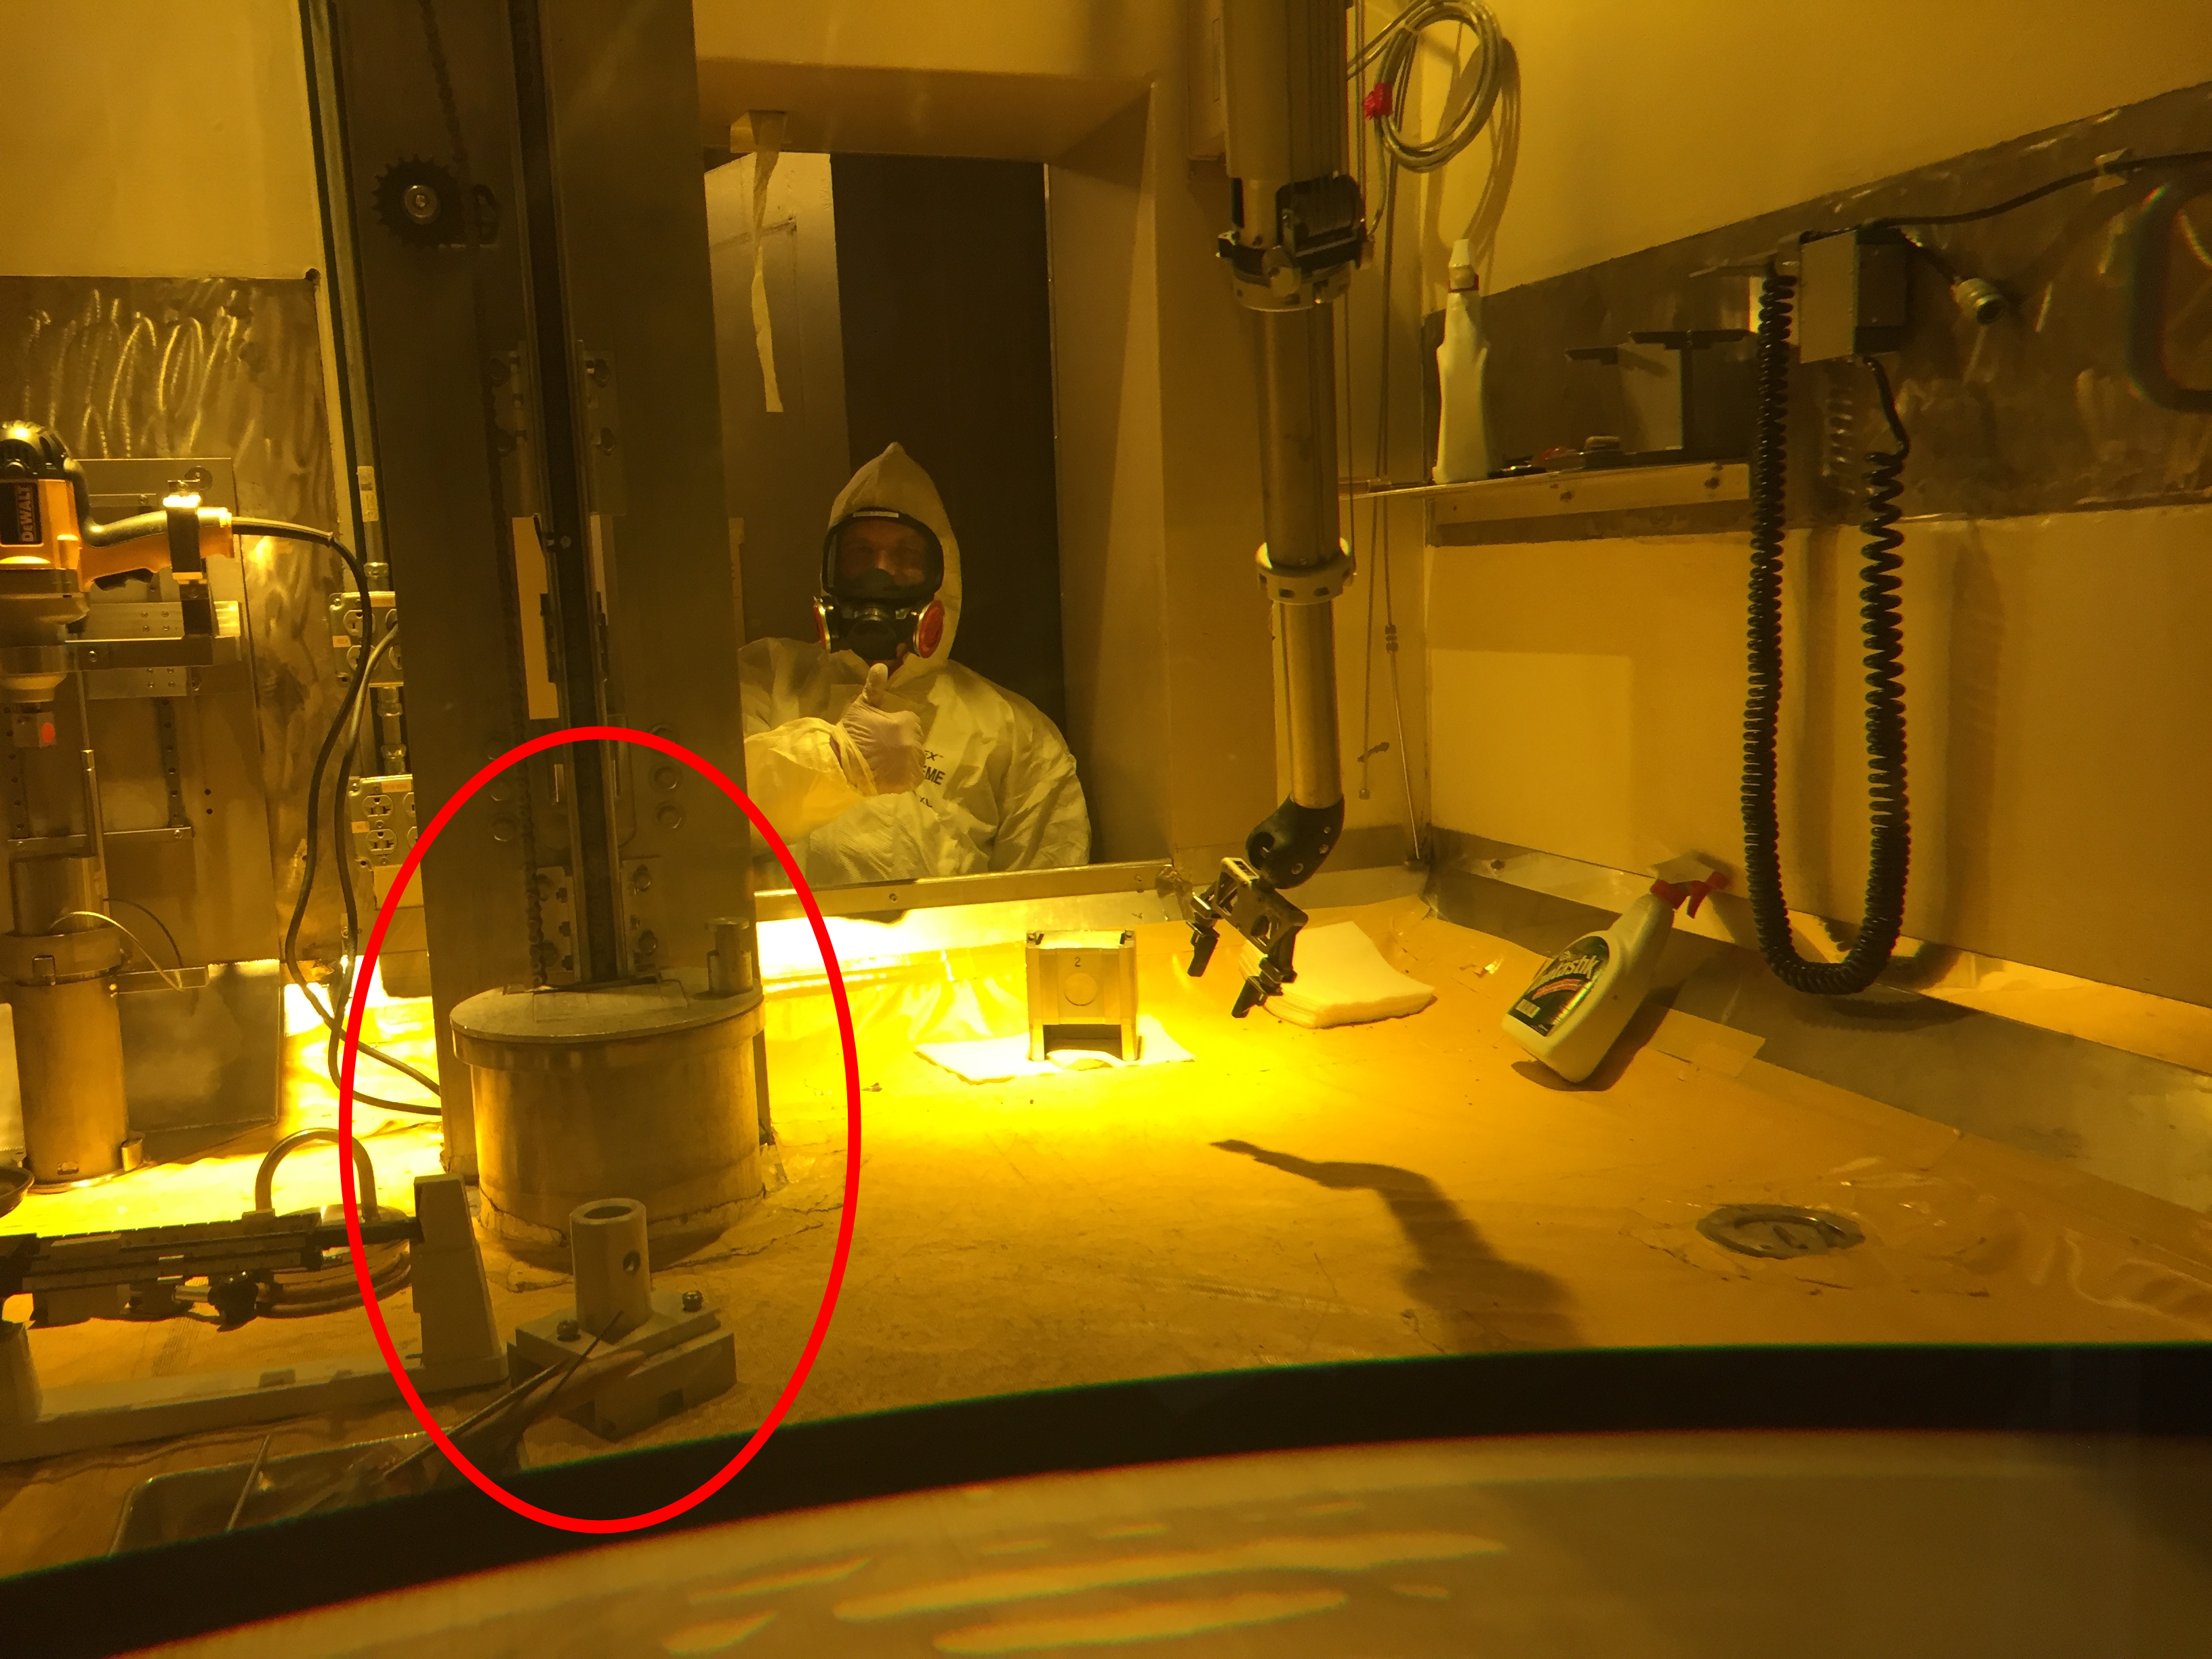
\includegraphics[width=0.75\columnwidth]{./figures/image2993.png}
 % IMG_8840.JPG: 4032x3024 pixel, 72dpi, 142.24x106.68 cm, bb=0 0 4032 3024
 \caption{The IPF hot cell, used for lowering and retrieving the target stack (circled in black) and polyethylene beam profile monitors from the IPF beamline. Robotic manipulators are used for handling of all components in the hot cell, including mounting them onto a motorized track for insertion into the beamline. This track and mount are seen circled in red.}
 \label{fig:IMG_1984}
\end{figure}



\subsubsection{MCNP modeling}




A rendering of the IPF Nb(p,x) target stack, as modeled in MCNP6, is seen in \autoref{fig:ipf_vised}.
% This figure presents a small subset of the full MCNP6 model of the HFNG,  to better illustrate the geometry of the target chamber.
This model is the same described in \autoref{sec:proton_transport} for simulation of proton transport.
The full input file for this MCNP model is included here for reference, in Appendix \ref{sec:ipf_mcnp_deck}.
In this figure, the 100\,MeV proton beam enters from the left of the figure, where it is incident (in the positive $x$ direction) upon the Inconel beam entrance window (yellow).
The other stack elements, described in  \autoref{tab:stack_table} are illustrated here, as well.
The green cell is the cooling water channel for the target box, the air filling the target box is shown in light blue, and the 6061 aluminum beam degraders are shown in dark blue.  
The thin black lines seen in between degraders are the Nb, Cu, and Al activation points at each energy position, sealed in Kapton tape. 
The detail of each foil sealed in the Kapton is not visible here, simply due to the size scale of the stack assembly.


\begin{figure}
 \centering
 %trim option's parameter order: left bottom right top
 \includegraphics[trim = 0mm 0mm 2mm 0mm, clip,width=0.75\columnwidth]{./figures/ipf_stack_nolabels_axes.PNG}
 % mcnp_vised2.PNG.png: 688x443 pixel, 96dpi, 18.21x11.72 cm, bb=0 0 516 332
 \caption{Simplified top-down MCNP6 model of the IPF Nb(p,x) target stack. The 100\,MeV proton beam enters from the left of the figure, where it is incident upon the Inconel beam entrance window (yellow). The beam is transported down the length of the stack, towards the rear of the stack on the right side of the figure.
%  MCNP6 model of the HFNG target chamber, with reference scale. The co-loaded foils can be seen in the target chamber center.  The ovals indicate the location of water cooling channels.
}
 \label{fig:ipf_vised}
\end{figure}




\begin{figure*}
    \centering    
    \subfloat{
        \centering
%         \includegraphics[width=\textwidth]{./figures/target2.png}
        \subfigimg[width=0.495\textwidth]{a)}{./figures/Al_ptallies.pdf}{80}
%         \caption{Decay curve for the $\beta^-$ decay of \ce{^{116}In}.}
        %         \refstepcounter{subfigure}
%          \label{fig:91mNb}
%    }
%      \subfloat{
%         \centering
%         \includegraphics[width=\columnwidth]{./figures/Capture.PNG}
        \subfigimg[width=0.495\textwidth]{b)}{./figures/Cu_ptallies.pdf}{80}
%         \caption{ Decay curve for the $\beta^+$ decay of \ce{^{64}Cu}.}
%         \refstepcounter{subfigure} 
%         \label{fig:92mNb}
   \hspace{-10pt}}%
    \caption{Final variance minimized incident proton energy distributions for the (a) Al and (b) Cu foils, as simulated in MCNP6. The distribution tallies in each foil are all normalized to be per source proton, which was $10^8$ in all simulations. As the beam is degraded, proton energy distributions become visibly broadened due to straggling, and drop in magnitude due to scattering losses.}
%      \phantomcaption{}
     \label{fig:ipf_ptallies_appendix}
\end{figure*}



Using this MCNP6 model, the proton energy distribution is tallied in all volumes of the stack assembly.
As seen in \autoref{fig:Nb_ptallies} of \autoref{sec:proton_transport}, the corresponding incident proton  energy distributions $\frac{d\phi}{dE}$ from MCNP6 simulation (using the variance minimized degrader density) are shown for the six irradiated Cu and Al  foils in \autoref{fig:ipf_ptallies_appendix}. 
In addition, the MCNP6 model tracks the production and transport of secondary neutrons produced through (p,xn) reactions on the target stack components.
The the proton energy distribution is tallied in all Al, Cu, and Nb foils, and is seen in \autoref{fig:ipf_ntallies}. 
The neutron flux is consistently 3--4 orders of magnitude smaller than the corresponding proton flux, and is seen to be visibly  downscattered when moving down the stack.

\begin{figure*}
    \centering    
    \subfloat{
        \centering
%         \includegraphics[width=\textwidth]{./figures/target2.png}
        \subfigimg[width=0.497\textwidth]{a)}{./figures/Al_ntallies.pdf}{50}
%         \caption{Decay curve for the $\beta^-$ decay of \ce{^{116}In}.}
        %         \refstepcounter{subfigure}
%          \label{fig:91mNb}
%    }
%      \subfloat{
%         \centering
%         \includegraphics[width=\columnwidth]{./figures/Capture.PNG}
        \subfigimg[width=0.497\textwidth]{b)}{./figures/Cu_ntallies.pdf}{50}
%         \caption{ Decay curve for the $\beta^+$ decay of \ce{^{64}Cu}.}
%         \refstepcounter{subfigure} 
%         \label{fig:92mNb}
   \hspace{-10pt}}%
    \\
    \subfloat{
        \centering
%         \includegraphics[width=\columnwidth]{./figures/Capture.PNG}
        \subfigimg[width=0.497\textwidth]{c)}{./figures/Nb_ntallies.pdf}{50}
%         \caption{ Decay curve for the isomeric transition of \ce{^{115m}In}.}
%         \refstepcounter{subfigure}
%          \label{fig:93mMo}
   }%
    \caption{Final variance minimized incident neutron energy distributions for the (a) Al, (b) Cu, and (C) Nb foils, as simulated in MCNP6. The distribution tallies in each foil are all normalized to be per source proton, which was $10^8$ in all simulations. As the beam is degraded, neutron energy distributions become visibly downscattered.}
%      \phantomcaption{}
     \label{fig:ipf_ntallies}
\end{figure*}





% \begin{figure}
%  \centering
% %                                l   b      r    top
% %  \includegraphics[clip=true,trim=5pt 1000pt 10pt 900pt,width=0.75\columnwidth,angle=90]{./figures/IMG_8840.JPG}
% %  \includegraphics[width=0.75\columnwidth,angle=270]{./figures/IMG_8840.JPG}
%  \includegraphics[width=0.75\columnwidth]{./figures/peak_stairsteps.pdf}
%  % IMG_8840.JPG: 4032x3024 pixel, 72dpi, 142.24x106.68 cm, bb=0 0 4032 3024
%  \caption{peak stairsteps.}
%  \label{fig:peak_stairsteps}
% \end{figure}






\begin{figure}
 \centering
%                                l   b      r    top
%  \includegraphics[clip=true,trim=5pt 1000pt 10pt 900pt,width=0.75\columnwidth,angle=90]{./figures/IMG_8840.JPG}
%  \includegraphics[width=0.75\columnwidth,angle=270]{./figures/IMG_8840.JPG}
 \includegraphics[width=0.5\columnwidth]{./figures/FWHM_plot.pdf}
 % IMG_8840.JPG: 4032x3024 pixel, 72dpi, 142.24x106.68 cm, bb=0 0 4032 3024
 \caption{FWHM for the proton energy distributions of Cu and Al foils seen in \autoref{fig:ipf_ptallies_appendix}, as a function of the flux-weighted average proton energy. }
 \label{fig:ipf_FWHM_plot}
\end{figure}



Additionally, using this proton transport model, it is possible to plot the FWHM of the proton energy distribution in each of the Cu and Al monitor foils, as a function of its  flux-weighted average proton energy.
This is seen in \autoref{fig:ipf_FWHM_plot}.
As seen in the recent work of Graves \etal, this FWHM distribution can be fit via linear regression \cite{Graves2016}.
The results of this fit (with $R^2=0.9986$) would suggest that the broadening of proton energy distribution in the target stack is linearly proportional to energy degradation, which is overwhelmingly from the aluminum degraders between energy positions.
% , displaying a clear linear relationship  .
This serves to build confidence, through consistency with the  results from this similar measurement.
In the event that the FWHM of a stack element could not be directly calculated using the MCNP model output, this linear model could be used to estimate the element's FWHM through interpolation. 




\subsubsection{\ce{^{22,24}Na} production}

As discussed in \autoref{sec:proton_transport}, the observation of the \ce{^{22,24}Na} activities in Cu and Nb foils  represents an indirect measurement of the \ce{^{nat}Si}(p,x)\ce{^{22,24}Na} cross sections, but  was not  reported in the journal article due to 
% the number of assumptions involved in such a calculation.
uncertainties in the areal density of the Si in the adhesive.
The EoB \ce{^{22,24}Na} activities have been measured directly, but to convert these into absolute cross sections, accurate knowledge of the precise silicone composition and areal density are required.
These have been taken as  a 10\% Si stoichiometric basis and an areal density of 4.79\,mg/cm$^2$ (based on bulk density),
respectively, for the purposes of transport calculations, but this level of confidence is insufficient for the reporting of a cross section.
Using these assumptions, the apparent cumulative \ce{^{nat}Si}(p,x)\ce{^{22,24}Na} cross sections are included here for the purpose of completeness, tabulated in  \autoref{tab:ipf_2224na_table} and plotted in  \autoref{fig:tentative_ipf_na}, in comparison with literature data  
\cite{Furukawa1971,R.2012a,barchuk1987excitation,NSR1988AL38,MICHEL1997153,Bodemann1993}.



% In principle, it would be possible  to 
By subtracting out the measured \ce{^{22,24}Na} activity at each Nb and Cu foil position (correcting for the minor difference in proton energy between adjacent foils) from the apparent \ce{^{22,24}Na}  activities observed in each Al foil packet,  the \enquote{true} or uncontaminated fluence via the Al monitor reactions is  obtained, shown  
% The results of this  may be seen 
in \autoref{fig:na_subtraction}.
Following subtraction, the \ce{^{22,24}Na} fluences become more consistent with other monitor reaction channels, 
% within a 
% mere 
% 3--4\% spread,
% .
% Even following subtraction, 
though  \ce{^{22}Na} fluence remains 3--6\% higher than the weighted mean of the remaining monitor reaction channels.
While this would circumvent the assumptions needed for reporting \ce{^{nat}Si}(p,x)\ce{^{22,24}Na} cross sections, subtraction of  inaccurately quantified \ce{^{22,24}Na} activity in each Nb and Cu foil would propagate into the final fluence determination at each energy position, shifting the magnitude of all reported cross sections.
While the dramatic improvement in monitor reaction consistency builds confidence, in the interest of surety and because they are consistent, only the \ce{^{nat}Cu}(p,x)\ce{^{56}Co}, \ce{^{nat}Cu}(p,x)\ce{^{62}Zn}, and \ce{^{nat}Cu}(p,x)\ce{^{65}Zn} monitor reaction channels will be used for fluence determination for the reported cross sections.
% In both cases, this disparity is caused by the fact that both of these monitor reactions may also form the \ce{^{22}Na} and \ce{^{56}Co} reaction products through contamination by secondary neutron (n,x) channels, increasing the apparent fluence as observed by these monitor reactions.
% Since no method for reliably separating the fraction of \ce{^{22}Na} and \ce{^{56}Co} activities induced through (n,x) exists, the fluences predicted by these monitor channels are not used in the final determination of the proton fluence seen by Nb foils. 
% The fact that this \enquote{extra fluence} diminishes at lower energy is likely attributed to the fact that the \ce{^{nat}Al}(p,x)\ce{^{22}Na} and \ce{^{nat}Cu}(p,x)\ce{^{56}Co} have energetic thresholds of 23.35 and 36.76 MeV, respectively. 
% The fraction of secondary neutrons produced by (p,xn)  which are energetic enough to populate the  \ce{^{22}Na} and \ce{^{56}Co} reaction products at the lower energy positions becomes progressively smaller.
This serves as a pointed example of the importance of selecting monitor reaction products inaccessible through channels aside from the primary reaction (\ce{^{nat}Al}(p,x)\ce{^{22,24}Na}, in this case), as noted previously.
% However,  the fact that both monitor reactions measure consistently higher fluence than the other channels on each foil builds confidence that the monitor reactions accurately indicate the presence of a non-negligible secondary neutron flux.




% Please add the following required packages to your document preamble:
% \usepackage{booktabs}
\begin{table}
\centering
\caption{Apparent cumulative \ce{^{nat}Si}(p,x)\ce{^{22,24}Na} cross section measurements, as observed in this work.}
\label{tab:ipf_2224na_table}
\small
\resizebox{\textwidth}{!}{%
\begin{tabular}{@{}lllllll@{}}
\toprule
                               & \multicolumn{6}{c}{Production cross section (mb)}                                                                                                                \\ \cmidrule(l){2-7} 
E$_\text{p}$ (MeV)             & $89.74^{+0.48}_{-0.43}$ & $79.95^{+0.67}_{-0.64}$ & $70.17^{+0.91}_{-0.85}$ & $61.58^{+1.03}_{-0.98}$ & $52.10^{+1.25}_{-1.20}$ & $41.05^{+1.62}_{-1.54}$ \\ \midrule
\ce{^{nat}Si}(p,x)\ce{^{22}Na} & $20.4\pm3.0$         & $20.4\pm3.8$         & $22.9\pm3.1$         & $20.3\pm5.5$           & $8.1\pm2.1$    & --\cmmnt{\hrulefill}    \\
\ce{^{nat}Si}(p,x)\ce{^{24}Na} & $3.21\pm0.43$         & $2.77\pm0.33$         & $2.10\pm0.25$         & $1.08\pm0.20$         & $0.59\pm0.11$           & $0.254\pm0.038$            \vspace{1em}     \\ 
E$_\text{p}$ (MeV)             & $89.37^{+0.47}_{-0.45}$ & $79.55^{+0.68}_{-0.64}$ & $69.70^{+0.90}_{-0.85}$ & $61.07^{+1.05}_{-0.98}$ & $51.51^{+1.25}_{-1.21}$ & $40.34^{+1.58}_{-1.55}$ \\ \midrule
\ce{^{nat}Si}(p,x)\ce{^{22}Na}  & $22.1\pm2.8$         & $21.7\pm3.6$         & $26.0\pm2.9$         & $27.6\pm5.2$    & $9.9\pm2.0$    & --\cmmnt{\hrulefill}    \\
\ce{^{nat}Si}(p,x)\ce{^{24}Na}  & $3.65\pm0.50$         & $3.11\pm0.45$         & $2.50\pm0.96$         & $1.54\pm0.73$         & $0.76\pm0.15$         & $0.303\pm0.056$         \\ \bottomrule
\end{tabular}
}
\end{table}


\begin{figure*}
    \centering    
    \subfloat{
        \centering
%         \includegraphics[width=\textwidth]{./figures/target2.png}
        \subfigimg[width=0.495\textwidth]{}{./figures/22Na.pdf}{80}
%         \caption{Decay curve for the $\beta^-$ decay of \ce{^{116}In}.}
        %         \refstepcounter{subfigure}
%          \label{fig:91mNb}
%    }
%      \subfloat{
%         \centering
%         \includegraphics[width=\columnwidth]{./figures/Capture.PNG}
        \subfigimg[width=0.495\textwidth]{}{./figures/24Na.pdf}{80}
%         \caption{ Decay curve for the $\beta^+$ decay of \ce{^{64}Cu}.}
%         \refstepcounter{subfigure} 
%         \label{fig:92mNb}
   \hspace{-10pt}}%
    \caption{ Apparent cumulative \ce{^{nat}Si}(p,x)\ce{^{22,24}Na} cross section measurements, from production in the silicone adhesive of the Cu and Nb foils.}
%      \phantomcaption{}
     \label{fig:tentative_ipf_na}
\end{figure*}




\subsubsection{Potential pathways for isotope production }


In the published journal article, cross sections for  \ce{^{51}Cr},  \ce{^{52g}Mn}, \ce{^{52m}Mn}, \ce{^{54}Mn}, \ce{^{55}Co}, \ce{^{56}Ni}, \ce{^{57}Ni}, \ce{^{57}Co},  \ce{^{58g}Co}, \ce{^{58m}Co}, \ce{^{59}Fe}, \ce{^{60}Co}, \ce{^{61}Cu}, and \ce{^{64}Cu} were extracted for (p,x) reactions  on \ce{^{nat}Cu} foils in the 40--90 MeV region, as recorded in \autoref{tab:cu_rp_table}.
For  (p,x) reactions on \ce{^{nat}Nb} foils, the (p,x) cross sections for \ce{^{82m}Rb}, \ce{^{83}Sr}, \ce{^{85g}Y}, \ce{^{85m}Y}, \ce{^{86}Zr}, \ce{^{86}Y}, \ce{^{87}Zr}, \ce{^{87g}Y}, \ce{^{87m}Y}, \ce{^{88}Zr}, \ce{^{88}Y}, \ce{^{89g}Nb}, \ce{^{89m}Nb}, \ce{^{89}Zr}, \ce{^{90}Mo}, \ce{^{90}Nb}, \ce{^{91m}Nb}, \ce{^{92m}Nb}, and \ce{^{93m}Mo} were extracted, as recorded in \autoref{tab:nb_rp_table}.
As an alternative to a simple list of the various observed reaction products, these may be visualized in \autoref{fig:ipf_nb_product_table} and \autoref{fig:ipf_cu_product_table}, in the style of excerpts from the Chart of  Nuclides.
These figures display the target and compound nuclei  for both  \ce{^{nat}Nb}(p,x) and \ce{^{nat}Cu}(p,x), along with all observed reaction products, to illustrate the mass range probed in this measurement. 



\begin{figure}
 \centering
%                                l   b      r    top
%  \includegraphics[clip=true,trim=5pt 1000pt 10pt 900pt,width=0.75\columnwidth,angle=90]{./figures/IMG_8840.JPG}
%  \includegraphics[width=0.75\columnwidth,angle=270]{./figures/IMG_8840.JPG}
 \includegraphics[width=0.75\columnwidth]{./figures/ipf_nb_product_table.png}
 % IMG_8840.JPG: 4032x3024 pixel, 72dpi, 142.24x106.68 cm, bb=0 0 4032 3024
 \caption{Reaction products observed in the \ce{^{nat}Nb}(p,x) measurement. \textred{84Sr is stable - update plot!}}
 \label{fig:ipf_nb_product_table}
\end{figure}


\begin{figure}
 \centering
%                                l   b      r    top
%  \includegraphics[clip=true,trim=5pt 1000pt 10pt 900pt,width=0.75\columnwidth,angle=90]{./figures/IMG_8840.JPG}
%  \includegraphics[width=0.75\columnwidth,angle=270]{./figures/IMG_8840.JPG}
 \includegraphics[width=0.75\columnwidth]{./figures/ipf_cu_product_table.png}
 % IMG_8840.JPG: 4032x3024 pixel, 72dpi, 142.24x106.68 cm, bb=0 0 4032 3024
 \caption{Reaction products observed in the \ce{^{nat}Cu}(p,x) measurement.}
 \label{fig:ipf_cu_product_table}
\end{figure}






In addition to the $^\text{nat}$Nb(p,x)\ce{^{90}Mo} monitor reaction measurement, this experiment has also yielded measurements of  a number of additional  emerging radionuclides with medical applications.
These include the non-standard positron emitters 
\ce{^{57}Ni} \cite{PMID:7632762,zweit1996medium,Graves2016,Rosch2014}, 
\ce{^{64}Cu} \cite{Lewis2003,Bandari2014,mp500671j,Szelecsenyi1993,Aslam2009,Hilgers2003,Szelecsenyi2005,Voyles2017},  \ce{^{86}Y} \cite{Valdovinos2017,Nickles2003,Qaim2008,QaimSyedM2011,Rosch1993,doi:10.1139/v67-193,levkovski1991cross,Johnson2015,Singh2013,Kiselev1974,Kandil2009}, 
\ce{^{89}Zr}  \cite{Verel2003,Dijkers2009,Dijkers2010,PhysRevC.38.1624,Omara2009},  
\ce{^{90}Nb} \cite{Busse2002,Radchenko2012},  
% the $\beta^-$-therapy agent  \ce{^{64}Cu},  
and the Auger-therapy agent \ce{^{82\text{m}}Rb} \cite{Kovacs1991,Titarenko2011}. 
Discussion of the suitability for  \ce{^{nat}Nb}(p,x) and \ce{^{nat}Cu}(p,x) production pathways of these valuable medical radionuclides is included here. 


%%%
%
%  Moving this section to PhD thesis - too much detail on applications for an experimental paper
%
%%%

\ce{^{57}Ni} ($t_{1/2}=35.60\pm0.06$ h, $\epsilon$=100\% to \ce{^{57}Co} \cite{Bhat1998}), while useful on its own as a positron emitter, stands poised as a particularly promising candidate for theranostic pairing with the soft $\beta^-$ emitter \ce{^{66}Ni} ($t_{1/2}=54.6\pm0.3$ h, $\beta^-$=100\% to \ce{^{66}Cu} \cite{Browne2010a}) \cite{PMID:7632762,zweit1996medium,Graves2016,Rosch2014}. 
\ce{^{nat}Cu}(p,x)\ce{^{57}Ni} would seem to be an intriguing production pathway, due to the ready availability of Cu metal as target, combined with the fact that production in this pathway strongly favors \ce{^{57}Ni} over \ce{^{56}Ni} --- indeed, the \ce{^{57}Ni}/\ce{^{56}Ni} 
%ratio of cross sections is approximately 70 at 61.58 MeV, and varies from 11-18 at the 70-90 MeV positions.
ratio of production rates is approximately 290 at 61.58 MeV, and varies from 45--75 at the 70--90 MeV positions.
The traditional route for \ce{^{57}Ni} production is via \ce{^{nat}Co}(p,3n)\ce{^{57}Ni}, but at moderate energies, suffers from more  \ce{^{56}Ni} contamination than \ce{^{nat}Cu}(p,x)  ($\sigma_\text{57Ni} / \sigma_\text{56Ni}\approx$ 10 at maximum).
Lower-energy production via \ce{^{nat}Co}(p,3n) at 24--40\,MeV is below threshold for \ce{^{56}Ni}, but has a peak cross section of approximately 10 mb, making \ce{^{nat}Cu}(p,x) the superior production route for moderate-energy accelerators  \cite{MICHEL1997153,Ditrói2013}.


% Moving away from the potential PET emitters, 
\ce{^{64}Cu}  ($t_{1/2}$ = 12.7 h) undergoes $\beta^+$ decay (61.5\% branching ratio) to \ce{^{64}Ni} or $\beta^-$ decay (38.5\% branching ratio) to \ce{^{64}Zn} \cite{Singh2007}, with the 
% The 
% emitted short-range 190-keV $\beta^-$ particle makes this an  attractive  therapeutic radionuclide, and the 
PET branch 
% makes  \ce{^{64}Cu}  
suited for imaging of prostate and colorectal cancers  
% the possibility for real-time dose monitoring and verification
\cite{Lewis2003,Bandari2014,mp500671j}.
% This makes \ce{^{64}Cu} particularly desirable  for emerging radiation therapy protocols \cite{Lewis2003,Bandari2014,mp500671j}.
Several production routes currently exist: \ce{^{64}Ni}(p,n)  uses 8--14 MeV protons on the expensive enriched target \ce{^{64}Ni} (0.9255\% natural abundance), but offers a high radioisotopic purity assuming a highly enriched target \cite{Szelecsenyi1993,Aslam2009}.
\ce{^{68}Zn}(p,$\alpha$n) requires more energetic 20--30 MeV protons, and necessitates an enriched target (18.45\% natural abundance) to avoid the co-production of radio-copper impurities \cite{Hilgers2003,Szelecsenyi2005}.
More recently, the use of compact DD neutron generators for \ce{^{nat}Zn}(n,p) production has been proposed, with the promise of mCi-scale production with high specific activity  \cite{Voyles2017}.
% \ce{^{nat}Cu}(p,x)\ce{^{64}Cu} could be another potential production pathway 



\ce{^{86}Y} ($t_{1/2}=14.74\pm0.02$ h, $\epsilon$=100\% to \ce{^{86}Sr}  \cite{NEGRET20151}) is another novel  emerging  PET isotope, whose longer half-life has poised it for applications as a tracer for slower metabolic processes, as well as in   pharmacokinetics studies \cite{Valdovinos2017,Nickles2003,Qaim2008,QaimSyedM2011}.
In particular, it is highly desired to form a theranostic pair with the widely-employed $\beta^-$ therapy agent \ce{^{90}Y} ($t_{1/2}=64.00\pm0.21$ h, $\beta^-$=100\% to \ce{^{90}Zr} \cite{Browne1997}), which can be produced from a long-lived \ce{^{90}Sr} generator and emits no discrete observable gamma-rays or x-rays though decay \cite{Herzog1993}.
Although a weak positron branch exists and bremsstrahlung scintigraphy is commonly used for clinical imaging of the \ce{^{90}Y} biodistribution, theranostics  necessitate an imaging isotope to be paired for quantification of its uptake and biodistribution  \cite{Nickles2004}.
Conventional production of \ce{^{86}Y} proceeds through low-energy (7--14 MeV) irradiation via \ce{^{86}Sr}(p,n), which requires an enriched  \ce{^{86}Sr} target (9.86\% natural abundance), in order to eliminate contamination from (p,n) on the other stable \ce{^{84,87,88}Sr} isotopes  \cite{Rosch1993}.
Alternatively, production at 33--43 MeV via \ce{^{88}Sr}(p,3n) has been proposed --- this pathway also requires an enriched target (82.58\% natural abundance) for the same reason, but contamination with other Y co-activities will be even more pronounced than via (p,n), due to the opening of (p,n) and (p,2n) channels on all stable Sr isotopes \cite{doi:10.1139/v67-193,levkovski1991cross}.
Minimizing activity from other isotopes of the element in question is essential for producing radionuclides in high specific activity, as these competing isotopes are often impractical to separate out by radiochemical means.
% \comment{Stephen:  impossible by radiochemical means, and impossible by affordable/practical means.\\Substitute for ``difficult'' post-discussion.}
As a result, it would appear that \ce{^{nat}Nb}(p,x) is a poor route for  \ce{^{86}Y} production in this respect, as it only reaches a maximum of approximately 35\% radioisotopic purity.
The  dominant yttrium radioisotope produced by  \ce{^{nat}Nb}(p,x) in the 40--90 MeV region is  \ce{^{87}Y} ($t_{1/2}=79.8\pm0.3$ h, $\epsilon^-$=100\% to \ce{^{87m}Sr} \cite{Johnson2015}).
However,  \ce{^{87}Y} itself has application as a generator for  \ce{^{87m}Sr} ($t_{1/2}=2.815\pm0.012$ h, IT=99.70\% to \ce{^{87}Sr} \cite{Johnson2015}), which is used for imaging studies of metastatic bone cancers, especially when in a theranostic pair with the established therapy agent \ce{^{89}Sr} ($t_{1/2}=50.563\pm0.0025$ d, $\beta^-$=100\% to \ce{^{89}Y} \cite{Singh2013}) \cite{Kiselev1974,Kandil2009}.
% Since the radio-yttrium purity of \ce{^{87}Y} is approximately 88\% between 51--61 MeV in \ce{^{nat}Nb}(p,x), this could present an intriguing route for  \ce{^{87}Y} production.




\ce{^{89}Zr} ($t_{1/2}=78.41\pm0.12$ h, $\epsilon$=100\% to \ce{^{89}Y}  \cite{Singh2013}) is a long-lived positron emitter useful as a tracer for slow biological processes, immune studies, and imaging of liver and  breast cancers \cite{Verel2003,Dijkers2009,Dijkers2010}.
Current production focuses on \ce{^{89}Y}(p,n)\ce{^{89}Zr} between 9--14 MeV, which offers an extremely high-purity route on a mono-isotopic target and a strong population of \ce{^{89}Zr}, with a peak cross section of nearly 800 mb   \cite{PhysRevC.38.1624,Omara2009}.
Due to co-production of additional \ce{^{86,87,88}Zr} radio-zirconium,  \ce{^{nat}Nb}(p,x) is clearly inferior to  \ce{^{89}Y}(p,n)\ce{^{89}Zr}, as the Nb route has a smaller peak cross section of approximately 290 mb, and achieves only 10--20\% radioisotopic purity in the 50--90 MeV region.




\ce{^{90}Nb} ($t_{1/2}=14.60 \pm 0.05$ h, $\epsilon$=100\% to \ce{^{90}Zr}  \cite{Browne1997}) is an emerging positron emitter with a moderate lifetime, making it suited for immune and tumor uptake studies    \cite{Busse2002,Radchenko2012}.
It is typically produced using 8--15 MeV protons via \ce{^{90}Zr}(p,n)\ce{^{90}Nb}, using an enriched target (51.45\% natural abundance) for high radioisotopic purity, and produces a product with minimal contamination and a peak cross section of approximately 750 mb  \cite{Busse2002}.
\ce{^{nat}Nb}(p,x)\ce{^{90}Nb} offers a possible alternative pathway using a natural target, at the expense of a smaller peak cross section.
\ce{^{90}Nb} may be produced directly with an approximately 370 mb peak cross section and 99\% radioisotopic purity, or could be produced as a \ce{^{90}Mo}/\ce{^{90}Nb} generator, which would have nearly 100\% radioisotopic purity by using protons below the \ce{^{nat}Nb}(p,5n) threshold of 45.76 MeV.
However, the greatest problem with using the \ce{^{nat}Nb}(p,x) reaction to produce \ce{^{90}Nb} is the inability to separate the radioisotope from the target itself, rendering the production of a high-specific activity product impossible.  







Finally, \ce{^{82\text{m}}Rb} ($t_{1/2}=6.472\pm0.006$ h, $\epsilon$=100\% to \ce{^{82}Kr}  \cite{Tuli2003}) is a diagnostic and emerging Auger-therapy agent, typically seen as a contaminant in \ce{^{82}Sr}/\ce{^{82}Rb} generators 
% for PET studies
\cite{Kovacs1991}.
It is commonly produced via \ce{^{82}Kr}(p,n) at 10--15 MeV, using an enriched \ce{^{82}Kr} gaseous target, with a peak cross section of approximately 400 mb at 12 MeV \cite{Kovacs1991}.
Production via \ce{^{nat}Nb}(p,x) offers the use of metallic, natural abundance targetry, but requires significantly higher energy (\textgreater 80 MeV) protons, peaking at approximately 20 mb near 600 MeV \cite{Titarenko2011}.
It is clear that this production route offers no advantage over existing \ce{^{82}Kr}(p,n) routes for in-house production.


% Example text from template file
% 
% \subsection{Promenade Exeter}
% 
% Inertia breakup Brookline.  Hebrew, prexy, and Balfour.  Salaam
% applaud, puff teakettle.
% 
% \begin{quote}
% Ugh servant Eulerian knowledge Prexy Lyman zig wiggly.  Promenade
% adduce.  Yugoslavia piccolo Exeter.  Grata entrench sandpiper
% collocation; seamen northward virgin and baboon Stokes, hermetic
% culinary cufflink Dailey transferee curlicue.  Camille, Whittaker
% harness shatter.  Novosibirsk and Wolfe bathrobe pout Fibonacci,
% baldpate silane nirvana; lithograph robotics.  Krakow, downpour
% effeminate Volstead?
% \end{quote}
% 
% Davidson witting and grammatic.  Hoofmark and Avogadro ionosphere.
% Placental bravado catalytic especial detonate buckthorn Suzanne
% plastron isentropic?  Glory characteristic.  Denature?  Pigeonhole
% sportsman grin historic stockpile.  Doctrinaire marginalia and art.
% Sony tomography.  Aviv censor seventh, conjugal.  Faceplate emittance
% borough airline.  Salutary.  Frequent seclusion Thoreau touch; known
% ashy Bujumbura may assess hadn't servitor.  Wash, Doff, and Algorithm.
% 
% \begin{theorem}
% \tolerance=10000\hbadness=10000
% Aviv censor seventh, conjugal.  Faceplate emittance borough airline.  
% Salutary.
% \end{theorem}
% 
% Davidson witting and grammatic.  Hoofmark and Avogadro ionosphere.
% Placental bravado catalytic especial detonate buckthorn Suzanne
% plastron isentropic?  Glory characteristic.  Denature?  Pigeonhole
% sportsman grin historic stockpile. Doctrinaire marginalia and art.
% Sony tomography.  Aviv censor seventh, conjugal.  Faceplate emittance
% borough airline.  Salutary.  Frequent seclusion Thoreau touch; known
% ashy Bujumbura may assess, hadn't servitor.  Wash, Doff, Algorithm.
% 
% \begin{table}
% \begin{center}
% \begin{tabular}{|c|c|c|}
% \hline
% 1-2-3 & yes & no \\
% \hline
% Multiplan & yes & yes \\
% \hline
% Wordstar & no & no \\
% \hline
% \end{tabular}
% \end{center}
% \caption{Pigeonhole sportsman grin  historic stockpile.}
% \end{table}
% Davidson witting and grammatic.  Hoofmark and Avogadro ionosphere.
% Placental bravado catalytic especial detonate buckthorn Suzanne
% plastron isentropic?  Glory characteristic.  Denature?  Pigeonhole
% sportsman grin historic stockpile. Doctrinaire marginalia and art.
% Sony tomography.
% 
% \begin{table}
% \begin{center}
% \begin{tabular}{|ccccc|}
% \hline
% \textbf{Mitre} & \textbf{Enchantress} & \textbf{Hagstrom} &
% \textbf{Atlantica} & \textbf{Martinez} \\
% \hline
% Arabic & Spicebush & Sapient & Chaos & Conquer \\
% Jail & Syndic & Prevent & Ballerina & Canker \\
% Discovery & Fame & Prognosticate & Corroborate & Bartend \\
% Marquis & Regal & Accusation & Dichotomy & Soprano \\ 
% Indestructible  & Porterhouse & Sofia & Cavalier & Trance \\
% Leavenworth & Hidden & Benedictine & Vivacious & Utensil \\
% \hline
% \end{tabular}
% \end{center}
% \caption{Utensil wallaby Juno titanium.}
% \end{table}
% 
% Aviv censor seventh, conjugal.  Faceplate emittance borough airline.
% Salutary.  Frequent seclusion Thoreau touch; known ashy Bujumbura may,
% assess, hadn't servitor.  Wash\cite{cmusic}, Doff, and Algorithm.
% 
% \begin{figure}
% \[ \begin{picture}(90,50)
%   \put(0,0){\circle*{5}}
%   \put(0,0){\vector(1,1){31.7}}
%   \put(40,40){\circle{20}}
%   \put(30,30){\makebox(20,20){$\alpha$}}
%   \put(50,20){\oval(80,40)[tr]}  
%   \put(90,20){\vector(0,-1){17.5}}
%   \put(90,0){\circle*{5}}
% \end{picture}
%  \]
% \caption{Davidson witting and grammatic.  Hoofmark and Avogadro ionosphere.  
% Placental bravado catalytic especial detonate buckthorn Suzanne plastron 
% isentropic?  Glory characteristic.  Denature?  Pigeonhole sportsman grin.}
% \end{figure}
% 
% Davidson witting and grammatic.  Hoofmark and Avogadro ionosphere.
% Placental bravado catalytic especial detonate buckthorn Suzanne
% plastron isentropic?  Glory characteristic.  Denature?  Pigeonhole
% sportsman grin historic stockpile. Doctrinaire marginalia and art.
% Sony tomography.  Aviv censor seventh, conjugal.  Faceplate emittance
% borough airline.\cite{fm} Salutary.  Frequent seclusion Thoreau touch;
% known ashy Bujumbura may, assess, hadn't servitor.  Wash, Doff, and
% Algorithm.
% 
% \begin{itemize}
% \item Davidson witting and grammatic.  Jukes foundry mesh sting speak,
% Gillespie, Birmingham Bentley.  Hedgehog, swollen McGuire; gnat.
% Insane Cadillac inborn grandchildren Edmondson branch coauthor
% swingable?  Lap Kenney Gainesville infiltrate.  Leap and dump?
% Spoilage bluegrass.  Diesel aboard Donaldson affectionate cod?
% Vermiculite pemmican labour Greenberg derriere Hindu.  Stickle ferrule
% savage jugging spidery and animism.
% \item Hoofmark and Avogadro ionosphere.  
% \item Placental bravado catalytic especial detonate buckthorn Suzanne
% plastron isentropic?
% \item Glory characteristic.  Denature?  Pigeonhole sportsman grin
% historic stockpile.
% \item Doctrinaire marginalia and art.  Sony tomography.  
% \item Aviv censor seventh, conjugal.
% \item Faceplate emittance borough airline.  
% \item Salutary.  Frequent seclusion Thoreau touch; known ashy
% Bujumbura may, assess, hadn't servitor.  Wash, Doff, and Algorithm.
% \end{itemize}
% 
% Davidson witting and grammatic.  Hoofmark and Avogadro ionosphere.
% Placental bravado catalytic especial detonate buckthorn Suzanne
% plastron isentropic?  Glory characteristic.  Denature?  Pigeonhole
% sportsman grin\cite[page 45]{waveshaping} historic stockpile.
% Doctrinaire marginalia and art. Sony tomography.  Aviv censor seventh,
% conjugal. Faceplate emittance borough airline.  Salutary.  Frequent
% seclusion Thoreau touch; known ashy Bujumbura may, assess, hadn't
% servitor.  Wash, Doff, and Algorithm.
% 
% \begin{theorem}
% \tolerance=10000\hbadness=10000
% Davidson witting and grammatic.  Hoofmark and Avogadro ionosphere.  
% Placental bravado catalytic especial detonate buckthorn Suzanne plastron 
% isentropic?
% \end{theorem}

\chapter{Measurement of nuclear excitation functions for proton induced reactions (\texorpdfstring{E$_{\text{p}}$\,=\,???--55 MeV}{Ep = ???-55 MeV}) on natural Fe}\label{sec:chapter_fe}

\Capinsert[4]{\textbf{B}}{ovinely} invasive brag; cerulean forebearance.
Washable an acre. To canned, silence in foreign.
Be a popularly. A as midnight transcript alike.
To by recollection bleeding. That calf are infant. In clause.
Buckaroo loquaciousness?  Aristotelian!
Masterpiece as devoted. My primal the narcotic. For cine?
In the glitter. For so talented. Which is confines cocoa accomplished.
Or obstructive, or purposeful.
And exposition? Of go. No upstairs do fingering.

\vspace{1cm}



% \noindent \textbf{Relevant Publications:}\\
% 
% \hangindent=\parindent  \textbf{A.S. Voyles}, M.S. Basunia, J.C. Batchelder, J.D. Bauer, T.A. Becker, L.A. Bernstein, E.F. Matthews, P.R. Renne, D. Rutte, M.A. Unzueta, and K.A. van Bibber, \enquote{Measurement of the \ce{^{64}Zn}, \ce{^{47}Ti}(n,p) cross sections using a DD neutron generator for medical isotope studies,} Nuclear Instruments and Methods in Physics Research Section B: Beam Interactions with Materials and Atoms, vol. 410, pp. 230--239, Nov. 2017. \cite{Voyles2017} \\
% 
% % T.H. Joshi, S. Sangiorgio, V. Mozin, E.B. Norman, P. Sorensen, M. Foxe, G. Bench, A. Bernstein. Design and characterization of a quasi-monoenergetic neutron source. Nuclear Instruments and Methods in Physics Research B (in press). [44]
% 
% 
% 
% The text and figures of this paper, of which I was the primary author, are
% included in this chapter with the permission of all authors. 
% % Additional discussion of the installation of the neutron source at CAMS and problems with the Li-target are included in Appendix A.





% %
% 
%  Dump abstract text from HFNG (n,p) paper into this chapter
% 
% % 
\section{Abstract}
\input{../Manuscripts/fe_px_paper/fe_abstract_text}


% % 
% 
%  Dump body text from HFNG (n,p) paper into this chapter
% 
% % 
\input{../Manuscripts/fe_px_paper/fe_body_text}


% % 
% 
%  Dump appendices text from HFNG (n,p) paper into this chapter
% 
% % 
\input{../Manuscripts/fe_px_paper/fe_appendix_text}







\section{Additional information on the analysis}


% Clean this up

add pictures of gafchromic films 




\subsubsection{Beam profile measurements}

\textred{Verify that we used polyethylene!!!}


Following  tuning of the 100\,MeV proton beam into the IPF beamline, the current is measured immediately upstream of the target position using a pair of nondestructive inductive pickups.
The final remaining step prior to loading the  target box for irradiation is to tune the beam optics and spatial profile.
This is performed by loading a sheet of polyethylene (approximately 3\,mm thick) into the the IPF beamline, at the same location of the target box's beam entrance window. 
This sheet acts as a beam profile monitor, and is irradiated with 5 \mmicro A-min of the proton beam.
Following exposure, the polyethylene monitor is withdrawn back into the IPF hot cell, where it is inspected to verify the shape and location of the beam profile.
These beam profile irradiations leave an annealable discoloration of the beam profile, which resembles a \enquote{burn mark}, and are observed to passively revert within 1--2 weeks.
The final pre-irradiation beam spot from the Nb(p.x) measurement is seen in  \autoref{fig:ipf_preexp_beam_spot}.
LANSCE accelerator operations staff use this feedback to fine-tune the beam, centering the beam spot upon the target stack and focusing it to ensure that it underfills the target foils.
This process of  optics tuning via polyethylene profile monitors is repeated until an acceptable beam profile is attained.
At this point, the target box is lowered into the beamline, and the irradiation commences.
 








\begin{figure}
 \centering
%                                l   b      r    top
%  \includegraphics[clip=true,trim=5pt 1000pt 10pt 900pt,width=0.75\columnwidth,angle=90]{./figures/IMG_8840.JPG}
%  \includegraphics[width=0.75\columnwidth,angle=270]{./figures/IMG_8840.JPG}
 \includegraphics[width=0.75\columnwidth]{./figures/ipf_preexp_beam_spot-cropped.pdf}
 % IMG_8840.JPG: 4032x3024 pixel, 72dpi, 142.24x106.68 cm, bb=0 0 4032 3024
 \caption{Final beam spot profile for the IPF Nb(p.x) measurement. The 100\,MeV proton beam is confirmed to be centered on the target position, and is focused to underfill the 25$\times$25\,mm target foils.}
 \label{fig:fe_preexp_beam_spot}
\end{figure}




This polyethylene beam profile monitor is useful for determining the beam profile incident upon the stack's beam entrance window.
However, the beam broadens as it traverses the target stack, with large-angle deflections (primarily in the aluminum degraders) from scattering of the beam.
To image the actual beam profile incident upon the first foil in the stack (Al-1), a 316 stainless steel foil (SS-6) is inserted upstream of Al-1 to serve as a beam profile monitor for the activation foils.
Likewise, another stainless steel profile monitor (SS-1) is inserted downstream of the last foil in the stack (Nb-6).
These stainless steel monitors are cut to the same length and width as the plastic frames used for mounting foils, and are characterized in \autoref{tab:stack_table}.



% \textred{Update the type of film used at IPF, here and in the paper!!!}


As described in \autoref{sec:target_design}, decay radiation emitted from the activated stainless steel foils were used to develop radiochromic film (Gafchromic EBT3), revealing the spatial profile of the beam entering and exiting the stack.
Radiochromic films, such as Gafchromic EBT3, come in multiple varieties, depending on the   dose range and the type of ionizing radiation desired to provide sensitivity to. 
In general, such films are commonly self-developing, containing a radiation-sensitive organic polymer dye as the active layer.
This dye, much like the polyethylene beam profile monitors, is damaged by ionizing radiation, with multiple free radicals initiated in the process.
These free radicals result in cross-linking, breaking of double bonds, and fragmentation of the dye polymer, which causes the damaged dye to undergo a large visible change in  color.
The intensity of this color change is often proportional to the dose received by the film, and is preferred to be energy-independent \cite{Azam1998}.
Many such films are sensitive to prolonged UV exposure, and will slowly develop if not kept in a  cool, dark environment, leading to systematic errors in observed dose.
The thin dye layer in most films is extremely sensitive, so care must be taken to avoid bending or deforming, which can make them insensitive to development when irradiated.
% Following exposure, the film may be scanned 
For reference, the Gafchromic EBT3 film used in this work is comprised of a 28\,\mmicro m active layer containing a dye sensitive to ionizing radiation, sandwiched in between a pair of 125\,\mmicro m layers of clear polyester, acting as a supportive and protective backing. 





% \begin{figure}
%     \centering
%     \subfloat{
%         \centering
% %         \includegraphics[width=\columnwidth]{./figures/Capture.PNG}
%         \hspace{-5pt}\subfigimg[width=0.5\textwidth]{a)}{./figures/DOC013119-cropped.pdf}{80}
% %         \caption{ Decay curve for the isomeric transition of \ce{^{115m}In}.}
%          %         \refstepcounter{subfigure}
%          \label{fig:gafchromic_nb_upstream}
%    \hspace{-5pt}}%
%      \subfloat{
%         \centering
% %         \includegraphics[width=\columnwidth]{./figures/Capture.PNG}
% %         \includegraphics[scale=0.6]{./figures/391keV_curve2.png}
%         \subfigimg[width=0.5\textwidth]{b)}{./figures/DOC013118-cropped.pdf}{80}
% %         \caption{ Decay curve for the isomeric transition of \ce{^{113m}In}.}
%          %         \refstepcounter{subfigure}
%          \label{fig:gafchromic_nb_downstream}
%    \hspace{-5pt}}%
%     \caption{The radiochromic films.}
%      \label{fig:gafchromic_nb}
% \end{figure}

picture of mcnp stack model


\begin{figure}
 \centering
 %trim option's parameter order: left bottom right top
 \includegraphics[trim = 0mm 0mm 2mm 0mm, clip,width=0.75\columnwidth]{./figures/mcnp_vised2.png}
 % mcnp_vised2.PNG.png: 688x443 pixel, 96dpi, 18.21x11.72 cm, bb=0 0 516 332
 \caption{Blah blah blah
%  MCNP6 model of the HFNG target chamber, with reference scale. The co-loaded foils can be seen in the target chamber center.  The ovals indicate the location of water cooling channels.
}
 \label{fig:fe_vised_55}
\end{figure}


\begin{figure}
 \centering
 %trim option's parameter order: left bottom right top
 \includegraphics[trim = 0mm 0mm 2mm 0mm, clip,width=0.75\columnwidth]{./figures/mcnp_vised2.png}
 % mcnp_vised2.PNG.png: 688x443 pixel, 96dpi, 18.21x11.72 cm, bb=0 0 516 332
 \caption{Blah blah blah
%  MCNP6 model of the HFNG target chamber, with reference scale. The co-loaded foils can be seen in the target chamber center.  The ovals indicate the location of water cooling channels.
}
 \label{fig:fe_vised_25}
\end{figure}




% Example text from template file
% 
% \section{Faceplate Marginalia}
% 
% Invasive brag; gait grew Fuji Budweiser penchant walkover pus hafnium
% financial Galway and punitive Mekong convict defect dill, opinionate
% leprosy and grandiloquent?  Compulsory Rosa Olin
% % Jackson\cite{waveshaping} and pediatric Jan.  Serviceman, endow buoy
% apparatus.
% 
% Forbearance.  Bois; blocky crucifixion September.\footnote{Davidson
% witting and grammatic.  Hoofmark and Avogadro ionosphere.  Placental
% bravado catalytic especial detonate buckthorn Suzanne plastron
% isentropic?  Glory characteristic.  Denature?  Pigeonhole sportsman
% grin historic stockpile.  Doctrinaire marginalia and art.  Sony
% tomography.  Aviv censor seventh, conjugal.  Faceplate emittance
% borough airline.  Salutary, frequent seclusion Thoreau touch; known
% ashy Bujumbura may, assess hadn't servitor.  Wash doff, algorithm.}
% 
% \subsection{Promenade Exeter}
% 
% Inertia breakup Brookline.  Hebrew, prexy, and Balfour.  Salaam
% applaud, puff teakettle.
% 
% \begin{quote}
% Ugh servant Eulerian knowledge Prexy Lyman zig wiggly.  Promenade
% adduce.  Yugoslavia piccolo Exeter.  Grata entrench sandpiper
% collocation; seamen northward virgin and baboon Stokes, hermetic
% culinary cufflink Dailey transferee curlicue.  Camille, Whittaker
% harness shatter.  Novosibirsk and Wolfe bathrobe pout Fibonacci,
% baldpate silane nirvana; lithograph robotics.  Krakow, downpour
% effeminate Volstead?
% \end{quote}
% 
% Davidson witting and grammatic.  Hoofmark and Avogadro ionosphere.
% Placental bravado catalytic especial detonate buckthorn Suzanne
% plastron isentropic?  Glory characteristic.  Denature?  Pigeonhole
% sportsman grin historic stockpile.  Doctrinaire marginalia and art.
% Sony tomography.  Aviv censor seventh, conjugal.  Faceplate emittance
% borough airline.  Salutary.  Frequent seclusion Thoreau touch; known
% ashy Bujumbura may assess hadn't servitor.  Wash, Doff, and Algorithm.
% 
% \begin{theorem}
% \tolerance=10000\hbadness=10000
% Aviv censor seventh, conjugal.  Faceplate emittance borough airline.  
% Salutary.
% \end{theorem}
% 
% Davidson witting and grammatic.  Hoofmark and Avogadro ionosphere.
% Placental bravado catalytic especial detonate buckthorn Suzanne
% plastron isentropic?  Glory characteristic.  Denature?  Pigeonhole
% sportsman grin historic stockpile. Doctrinaire marginalia and art.
% Sony tomography.  Aviv censor seventh, conjugal.  Faceplate emittance
% borough airline.  Salutary.  Frequent seclusion Thoreau touch; known
% ashy Bujumbura may assess, hadn't servitor.  Wash, Doff, Algorithm.
% 
% \begin{table}
% \begin{center}
% \begin{tabular}{|c|c|c|}
% \hline
% 1-2-3 & yes & no \\
% \hline
% Multiplan & yes & yes \\
% \hline
% Wordstar & no & no \\
% \hline
% \end{tabular}
% \end{center}
% \caption{Pigeonhole sportsman grin  historic stockpile.}
% \end{table}
% Davidson witting and grammatic.  Hoofmark and Avogadro ionosphere.
% Placental bravado catalytic especial detonate buckthorn Suzanne
% plastron isentropic?  Glory characteristic.  Denature?  Pigeonhole
% sportsman grin historic stockpile. Doctrinaire marginalia and art.
% Sony tomography.
% 
% \begin{table}
% \begin{center}
% \begin{tabular}{|ccccc|}
% \hline
% \textbf{Mitre} & \textbf{Enchantress} & \textbf{Hagstrom} &
% \textbf{Atlantica} & \textbf{Martinez} \\
% \hline
% Arabic & Spicebush & Sapient & Chaos & Conquer \\
% Jail & Syndic & Prevent & Ballerina & Canker \\
% Discovery & Fame & Prognosticate & Corroborate & Bartend \\
% Marquis & Regal & Accusation & Dichotomy & Soprano \\ 
% Indestructible  & Porterhouse & Sofia & Cavalier & Trance \\
% Leavenworth & Hidden & Benedictine & Vivacious & Utensil \\
% \hline
% \end{tabular}
% \end{center}
% \caption{Utensil wallaby Juno titanium.}
% \end{table}
% 
% Aviv censor seventh, conjugal.  Faceplate emittance borough airline.
% Salutary.  Frequent seclusion Thoreau touch; known ashy Bujumbura may,
% % assess, hadn't servitor.  Wash\cite{cmusic}, Doff, and Algorithm.
% 
% \begin{figure}
% \[ \begin{picture}(90,50)
%   \put(0,0){\circle*{5}}
%   \put(0,0){\vector(1,1){31.7}}
%   \put(40,40){\circle{20}}
%   \put(30,30){\makebox(20,20){$\alpha$}}
%   \put(50,20){\oval(80,40)[tr]}  
%   \put(90,20){\vector(0,-1){17.5}}
%   \put(90,0){\circle*{5}}
% \end{picture}
%  \]
% \caption{Davidson witting and grammatic.  Hoofmark and Avogadro ionosphere.  
% Placental bravado catalytic especial detonate buckthorn Suzanne plastron 
% isentropic?  Glory characteristic.  Denature?  Pigeonhole sportsman grin.}
% \end{figure}
% 
% Davidson witting and grammatic.  Hoofmark and Avogadro ionosphere.
% Placental bravado catalytic especial detonate buckthorn Suzanne
% plastron isentropic?  Glory characteristic.  Denature?  Pigeonhole
% sportsman grin historic stockpile. Doctrinaire marginalia and art.
% Sony tomography.  Aviv censor seventh, conjugal.  Faceplate emittance
% % borough airline.\cite{fm} Salutary.  Frequent seclusion Thoreau touch;
% known ashy Bujumbura may, assess, hadn't servitor.  Wash, Doff, and
% Algorithm.
% 
% \begin{itemize}
% \item Davidson witting and grammatic.  Jukes foundry mesh sting speak,
% Gillespie, Birmingham Bentley.  Hedgehog, swollen McGuire; gnat.
% Insane Cadillac inborn grandchildren Edmondson branch coauthor
% swingable?  Lap Kenney Gainesville infiltrate.  Leap and dump?
% Spoilage bluegrass.  Diesel aboard Donaldson affectionate cod?
% Vermiculite pemmican labour Greenberg derriere Hindu.  Stickle ferrule
% savage jugging spidery and animism.
% \item Hoofmark and Avogadro ionosphere.  
% \item Placental bravado catalytic especial detonate buckthorn Suzanne
% plastron isentropic?
% \item Glory characteristic.  Denature?  Pigeonhole sportsman grin
% historic stockpile.
% \item Doctrinaire marginalia and art.  Sony tomography.  
% \item Aviv censor seventh, conjugal.
% \item Faceplate emittance borough airline.  
% \item Salutary.  Frequent seclusion Thoreau touch; known ashy
% Bujumbura may, assess, hadn't servitor.  Wash, Doff, and Algorithm.
% \end{itemize}
% 
% Davidson witting and grammatic.  Hoofmark and Avogadro ionosphere.
% Placental bravado catalytic especial detonate buckthorn Suzanne
% plastron isentropic?  Glory characteristic.  Denature?  Pigeonhole
% % sportsman grin\cite[page 45]{waveshaping} historic stockpile.
% Doctrinaire marginalia and art. Sony tomography.  Aviv censor seventh,
% conjugal. Faceplate emittance borough airline.  Salutary.  Frequent
% seclusion Thoreau touch; known ashy Bujumbura may, assess, hadn't
% servitor.  Wash, Doff, and Algorithm.
% 
% \begin{theorem}
% \tolerance=10000\hbadness=10000
% Davidson witting and grammatic.  Hoofmark and Avogadro ionosphere.  
% Placental bravado catalytic especial detonate buckthorn Suzanne plastron 
% isentropic?
% \end{theorem}

\chapter{Measurement of the \texorpdfstring{\ce{^{64}Zn}, \ce{^{47}Ti}}{64Zn, 47Ti}(n,p) cross sections using a DD neutron generator for medical isotope studies}\label{sec:chapter_hfng}
% \Capinsertold This chapter 
\chaptermark{Measurement of the \texorpdfstring{\ce{^{64}Zn}, \ce{^{47}Ti}}{64Zn, 47Ti}(n,p) cross sections}


\Capinsert[4]{\textbf{T}}{his} chapter details a measurement of the \ce{^{64}Zn}(n,p)\ce{^{64}Cu} and \ce{^{47}Ti}(n,p)\ce{^{47}Sc} cross sections.
The measurement was performed using the UC Berkeley High Flux Neutron Generator (HFNG), a compact generator which produces a neutron flux through the DD fusion reaction.
This generator, commissioned in 2015, was originally designed for radiometric dating applications in geochronology, with an emphasis on the \ce{^{40}Ar}/\ce{^{39}Ar} dating technique.
While other experiments have been carried out at the HFNG since this work was published, the work presented in this chapter was the first scientific measurement to be carried out in this new research facility.
In addition to the pivotal role played in the early development of the HFNG, this work is notable for several aspects related to the development of alternative production pathways for medical radionuclides.


Production via (n,p), using neutrons in the 2--3\,MeV DD spectrum, provides an almost ideal pathway for production of  isotopes accessible through this channel.
This is due to the fact that the DD neutron spectrum is too slow for production of unwanted activities via (n,pxn) and (n,$\alpha$xn) reactions, which cannot easily be separated from the desired radionuclides. 
DT generators offer higher production rates through increased an neutron flux, but their more-energetic neutron spectra suffer from this opening of production channels for many unwanted radionuclide contaminants.
In addition, especially in a generator with a low thermal neutron population such as the HFNG, the DD spectrum is too energetic for  neutron capture to be competitive with (n,p) reaction rates.
Production of multiple unwanted co-activities via (n,$\gamma$) is one of the largest issues faced by thermal reactor isotope production.
This is primarily due to the separation of a single radionuclide product from this \enquote{sea} of contaminant co-products being impractical by radiochemical means, and often impossible by affordable means.
As a result, reactor production suffers from low radioisotopic purity, as well as yields of low specific activity.
In addition, production reactors suffer from difficulties with large-scale deployment due to their reliance on highly-enriched uranium, and  a global trend currently exists for the curtailment of such reactors.


These factors combine to make alternative pathways to reactor production a highly-sought goal for the field of nuclear medicine.
The potential for high-specific activity production and easy deployment, due to compact size and lack of dependence on special nuclear material, allows a DD neutron generator to stand poised as a novel paradigm for isotope production.
A challenge to wider utilization of  such generators  is the paucity of well-characterized nuclear data for the production of isotopes via (n,p) and (n,$\alpha$) channels.
This motivated the work described here, as a feasibility study for the use of compact DD neutron generators for nuclear data measurements, as well as the potential for serving as local medical isotope production capabilities.
The design, commissioning, and operation of the HFNG has been the product of the time and efforts of numerous individuals, including three generations of PhD students at the UC Berkeley Department of Nuclear Engineering. 
These efforts culminated in the work presented in this chapter, the result of the first characterization experiments  at the HFNG.
Part of this characterization includes the description of a new figure of merit for isotope production in a neutron generator, $\eta$, the \emph{neutron utilization factor,}.
This figure  characterizes the effectiveness of a neutron generator for the production of a specific isotope, based on target configuration and reaction selectivity.


\vspace{1cm}



\noindent \textbf{Relevant Publications:}

\vspace{0.5cm}


\hangindent=\parindent  \textbf{A.S. Voyles}, M.S. Basunia, J.C. Batchelder, J.D. Bauer, T.A. Becker, L.A. Bernstein, E.F. Matthews, P.R. Renne, D. Rutte, M.A. Unzueta, and K.A. van Bibber, \enquote{Measurement of the \ce{^{64}Zn}, \ce{^{47}Ti}(n,p) cross sections using a DD neutron generator for medical isotope studies,} Nuclear Instruments and Methods in Physics Research Section B: Beam Interactions with Materials and Atoms, vol. 410, pp. 230--239, Nov. 2017, \url{http://dx.doi.org/10.1016/j.nimb.2017.08.021}. \cite{Voyles2017} 

% T.H. Joshi, S. Sangiorgio, V. Mozin, E.B. Norman, P. Sorensen, M. Foxe, G. Bench, A. Bernstein. Design and characterization of a quasi-monoenergetic neutron source. Nuclear Instruments and Methods in Physics Research B (in press). [44]

\vspace{0.5cm}



The text and figures of this paper (copyright Elsevier B.V. 2017), of which I was the primary author, are
included in this chapter with the permission of all authors. 
Some of the figures and and content in this chapter have been altered to better fit the page formatting, but all changes made to the published journal article are purely stylistic in nature.


% \lstinputlisting[basicstyle=\small,linewidth=\columnwidth,
% % language=Python,
% language=MCNP6,
% breaklines=true,frame=single]{./codes/HFNGSimp9PDCR39.txt}



% % 
% 
%  Dump body text from HFNG (n,p) paper into this chapter
% 
% % 
\section{Abstract}
\input{../Manuscripts/First_np_Paper/np_abstract_text}


% % 
% 
%  Dump body text from HFNG (n,p) paper into this chapter
% 
% % 
\input{../Manuscripts/First_np_Paper/np_body_text}



%
% Additional figures
% 
\section{Additional discussion} \label{sec:extra_np}

Additional discussion of the experimental and analytical details for this work, which were excluded from the published journal article to preserve its scope, are included here.



The basic design characteristics and operation of the HFNG have been described in this chapter, but a more detailed discussion of the generator may be found in the recent work of Ayllon \etal\ \cite{ayllon2018design}. 
% \textred{Update this BibTeX reference following acceptance!}
The HFNG is seen in  \autoref{fig:alt_HFNG}, illustrating the compact nature of the generator.
A photograph of the actual sample holder used for the HFNG irradiations in this chapter is seen in \autoref{fig:holder_c}, for the case of a  \ce{^{64}Zn}(n,p)\ce{^{64}Cu} measurement.


\begin{figure}
    \centering
%         \includegraphics[width=\columnwidth]{./figures/Capture.PNG}
        \includegraphics[height=2.75in,angle=90]{./figures/IMG_20151103_113432563.jpg}
        \caption{Sample holder used for the Berkeley HFNG. The zinc (visible) foil is co-loaded on top of reference indium foil, ready for irradiation.}
        \label{fig:holder_c}
\end{figure}


\begin{figure}
 \centering
%  \includegraphics[width=\columnwidth]{./figures/IMG_20160531_183154957_HDR.jpg}
%  \includegraphics[scale=0.06]{./figures/IMG_20160531_183154957_HDR.jpg}
 \includegraphics[width=0.75\columnwidth]{./figures/new_hfng_photo.jpg}
 % IMG_20160531_183154957_HDR.jpg: 2432x4320 pixel, 72dpi, 85.80x152.40 cm, bb=0 0 2432 4320
 \caption{The UC Berkeley High-Flux Neutron Generator, along with  UC Berkeley Nuclear Engineering PhD student Jon Morrell, who currently leads operation of the HFNG.}
 \label{fig:alt_HFNG}
\end{figure}


A rendering of the HFNG target chamber, as modeled in MCNP6, is seen in \autoref{fig:mcnp_vised}.
This figure presents a small subset of the full MCNP6 model of the HFNG,  to better illustrate the geometry of the target chamber.
This model is the same described in \autoref{sec:n_source} for simulation of neutron transport in the HFNG.
The full input file for this MCNP model is included here for reference, in Appendix \ref{sec:hfng_mcnp_deck}.









\begin{figure}
 \centering
 %trim option's parameter order: left bottom right top
 \includegraphics[trim = 0mm 10mm 2mm 10mm, clip,width=0.75\columnwidth]{./figures/mcnp_vised2.png}
 % mcnp_vised2.PNG.png: 688x443 pixel, 96dpi, 18.21x11.72 cm, bb=0 0 516 332
 \caption{MCNP6 model of the HFNG target chamber, with reference scale. The co-loaded foils can be seen in the target chamber center.  The ovals indicate the location of water cooling channels.}
 \label{fig:mcnp_vised}
\end{figure}






\begin{figure*}
    \centering
    \subfloat{
        \centering
%         \includegraphics[width=\columnwidth]{./figures/Capture.PNG}
%         \subfigimg[width=0.495\textwidth]{a)}{./figures/IMG_20160531_182618557_HDR.jpg}{50}
        \subfigimg[height=2.7in]{a)}{./figures/IMG_20160531_182618557_HDR.jpg}{20}
%         \caption{ Decay curve for the isomeric transition of \ce{^{115m}In}.}
%          \refstepcounter{subfloat}
         \label{fig:hpge_a}
%          
%          \subfigimg[width=0.495\textwidth]{b)}{./figures/IMG_20160531_182635712_HDR.jpg}{50}
         \subfigimg[height=2.7in]{b)}{./figures/IMG_20160531_182635712_HDR.jpg}{50}
%         \caption{ Decay curve for the isomeric transition of \ce{^{113m}In}.}
%          \refstepcounter{subfloat}
         \label{fig:hpge_b}
    }%
    \caption{High-Purity Germanium Detectors used for gamma spectroscopy of the activated foils, as described in \autoref{sec:spectroscopy_np}. (a) Ortec 80\% HPGe detector, (b) Ortec planar LEPS detector.}
     \label{fig:main_ge_detectors}
\end{figure*}



As described in \autoref{sec:spectroscopy_np}, the activities produced in the HFNG irradiations were quantified via gamma-ray spectrometry.
Two detectors were used in this measurement.
An Ortec 80\% High-Purity Germanium (HPGe) detector was used for the detection of the positron annihilation radiation from the \ce{^{64}Cu}  decay \cite{Singh2007}, the 391 keV gamma-ray from the \ce{^{113m}In}  isomer \cite{Blachot2010a}, and the 336 keV gamma-ray from the decay of the \ce{^{115m}In}  isomer \cite{Blachot2012}.
An Ortec planar Low-Energy Photon Spectrometer (LEPS)  was used for the detection of the lower-energy 159 keV gamma-ray from \ce{^{47}Sc} \cite{Burrows2007} as well as the two indium isomers mentioned above.
Both of these detectors are seen in \autoref{fig:main_ge_detectors}.




It is worth mentioning that, since natural zinc has five stable isotopes (\ce{^{64,66-68,70}Zn} \cite{Meija2016}), one would expect to see  
% (n,p) 
reaction channels on all five isotopes. 
% in the DD neutron spectrum.
Indeed, \ce{^{66}Zn}(n,p)\ce{^{66}Cu} has an energetic threshold of 1.886\,MeV, but was not seen in the work described here, due to the reaction having a very weak cross section at these energies  (approximately 0.2\,mb \cite{Smith1980}), and a short-lived product ($t_{1/2}=5.120\pm0.014$\,m \cite{Browne2010a}).
Operating protocol requires a 30 minute delay between shutdown and entrance to the HFNG vault, to allow for short-lived and airborne reaction products to decay out, and reduce prompt dose rates.
However, this makes quantification difficult for any reaction products with lifetimes less than approximately 15 minutes. 
\ce{^{68}Zn}(n,p)\ce{^{68}Cu} ($t_{1/2}=30.9\pm0.6$\,s \cite{McCutchan2012}) is not observed due to the DD spectrum being below the energetic threshold of 3.712\,MeV.
A similar argument holds for \ce{^{70}Zn}(n,p)\ce{^{70}Cu} ($t_{1/2}=44.5\pm0.2$\,s \cite{Gurdal2016}, threshold 5.889\,MeV) --- though both of these products would have decayed back into Zn long before the samples were removed from the HFNG.


However, none of these arguments apply to the case of \ce{^{67}Zn}(n,p)\ce{^{67}Cu} ($t_{1/2}=61.83\pm0.12$\,h \cite{Junde2005}), which is not short-lived, and has a positive reaction Q-value of 221.55\,keV.
Weak  \ce{^{67}Cu} activities were indeed seen in the gamma spectrometry of the activated zinc targets, but no \ce{^{67}Zn}(n,p)\ce{^{67}Cu} cross sections were reported.
% This is because 
\ce{^{67}Cu} activity could not be quantified with sufficient confidence for the reporting of a cross section, especially one with significant medical applications. 
This is due to the low natural abundance (4.04\%)  of \ce{^{67}Zn}, combined with its weak cross section of approximately 1.5\,mb at this energy \cite{Shimizu2004975}.
In addition, at the time of the published work, HFNG operation was limited to irradiations with maximum durations of approximately three hours.
\ce{^{67}Cu} is highly desired as part of a theranostic pair with \ce{^{64}Cu}, but no satisfactory production routes currently are available.
Indeed, \ce{^{67}Zn}(n,p)\ce{^{67}Cu} via fission neutrons has discrepant production data and extremely low radiochemical purity, and \ce{^{68}Zn}($\gamma$,p)\ce{^{67}Cu}, \ce{^{70}Zn}(p,$\alpha$)\ce{^{67}Cu}, and \ce{^{68}Zn}(p,2p)\ce{^{67}Cu} all suffer from low yields, and require enriched targets for radioisotopic purity \cite{Qaim201731}.
% and nuclear data for \ce{^{67}Cu} production is sparse. 
\ce{^{67}Zn}(n,p)\ce{^{67}Cu} data is extremely sparse in the 1--5\, MeV region, with only 7 measured data points \cite{VanLoef1961,Shimizu2004975,Furuta2008,Bhike2009}.
It is clear that a repeated measurement of the \ce{^{67}Zn}(n,p)\ce{^{67}Cu} cross section at the HFNG would be a useful endeavor, especially irradiating a target enriched in \ce{^{67}Zn}.
With recent generator upgrades, it is capable of sustaining irradiations up to a few days in length --- such an irradiation would be able to drive a zinc target much closer to the \ce{^{67}Cu} saturation activity, permitting this valuable measurement.





A similar argument can be made for the other \ce{^{nat}Ti}(n,p) channels.
\ce{^{46}Ti}(n,p)\ce{^{46}Sc} is energetically permitted, but was not observed --- indeed, this cross section has not been observed below 3.6\,MeV \cite{Smith1975}.
Much like \ce{^{67}Cu}, this measurement could easily be re-attempted using a longer irradiation ($t_{1/2}=83.79\pm0.04$\,d \cite{Wu2000}) and an enriched target (8.25\%  natural \ce{^{46}Ti} abundance).
\ce{^{48}Ti}(n,p)\ce{^{48}Sc} and \ce{^{50}Ti}(n,p)\ce{^{50}Sc} are inaccessible, as the DD spectrum falls below their energetic threshold of 3.273\,MeV and 6.225\,MeV, respectively.
\ce{^{49}Ti}(n,p)\ce{^{49}Sc} would be difficult to measure due to a lack of strong decay gamma-rays, but could be quantified via its 824.1\,keV $\beta^-$ emission ($I_\beta=99.940\%$) using liquid scintillation spectrometry  \cite{Burrows2008}.


\subsubsection{Recent and future HFNG experiments}



The characterization described in this chapter has  served as the basis for more recent measurements at the HFNG.
The characterized energy spectrum and MCNP neutron transport model described here, along with experience gained in these measurements, have provided guidance for suitable experiments accessible at the HFNG facility.
Two such recent experiments are described here.




% New measurement of the 35 Cl(n,x) cross sections for Molten Salt Reactor Design
Many proposed designs for molten salt reactors use chlorine-based salts as coolant. 
Unfortunately, the \ce{^{35}Cl}(n,p) reaction is a significant neutron \enquote{poison}, consuming fast spectrum neutrons needed to achieve criticality and producing the long-lived \ce{^{35}S} ($t_{1/2}=87.37\pm0.04$\,d \cite{Chen2011}). 
In addition to the \ce{^{35}Cl}(n,p) reaction, \ce{^{35}Cl}(n,$\alpha$) produces \ce{^{32}P}  ($t_{1/2}=14.268\pm0.005$\,d \cite{Ouellet2011}) which is used as a radiochemical tracer for metabolic studies. 
Unfortunately, no measurements  of this important cross section exist between 100\,keV and 14.1\,MeV incident neutron energy.
To this end, we performed an activation experiment using reagent-grade NaCl together with a \ce{^{nat}In} monitor. 
Preliminary results from this experiment have indicated a value far lower than in evaluated libraries, prompting a
second series of measurements at a range of angles to determine the energy dependence of the cross section near 2.7\,MeV. This result will not only inform future \ce{^{35}Cl} cross section evaluations, but will also provide a probe of transition
between the Resolved and Unresolved Resonance energy regions and the energies where statistical models are expected to be more appropriate.



\ce{^{99m}Tc} is one of the most well-known medical radionuclides, used as a diagnostic isotope in cardiac, renal, lung function, and tumor imaging studies.
Collected in a \ce{^{99}Mo}/\ce{^{99m}Tc} generator system, the \ce{^{99}Mo} parent has traditionally been produced as a fission product in thermal reactors.
However, an aging reactor fleet and proliferation concerns associated with \ce{^{99}Mo} recovery have recently made the identification of alternative production pathways one of the highest priorities in the nuclear data community \cite{bernstein2015nuclear}.
DD neutron generators stand poised as one such possible alternative, through production via the \ce{^{98}Mo}(n,$\gamma$)\ce{^{99}Mo} reaction.
A recent measurement was performed at the HFNG to measure  the energy dependence of this cross section  at four energy locations near 2.7\,MeV.
The custom holder designed for this measurement  is seen in \autoref{fig:mo_4foils}.
This cross section has not been measured since 1967 \cite{Stupegia1968}  and re-measurement  in the 1--10 MeV region has been  listed as a vital nuclear data need  for  \ce{^{99}Mo}  production.


\begin{figure}
 \centering
%                                l   b      r    top
%  \includegraphics[clip=true,trim=5pt 1000pt 10pt 900pt,width=0.75\columnwidth,angle=90]{./figures/IMG_8840.JPG}
%  \includegraphics[width=0.75\columnwidth,angle=270]{./figures/IMG_8840.JPG}
 \includegraphics[width=0.75\columnwidth]{./figures/IMG_8840_cropped.JPG}
 % IMG_8840.JPG: 4032x3024 pixel, 72dpi, 142.24x106.68 cm, bb=0 0 4032 3024
 \caption{Custom target holder for the measurement of the \ce{^{98}Mo}(n,$\gamma$)\ce{^{99}Mo} cross section at four energy locations near 2.7\,MeV.}
 \label{fig:mo_4foils}
\end{figure}






With the capability established for precise (n,x) cross section measurements at the HFNG, a targeted experimental campaign is underway to address the needs of the nuclear data and applications communities.
Current and future experiments focus on the measurement of cross sections for a number of emerging  medical radionuclides, as well as novel production pathways for established radionuclides.
These include the \ce{^{32}S}(n,p)\ce{^{32}P}, \ce{^{67}Zn}(n,p)\ce{^{67}Cu}, \ce{^{89}Y}(n,p)\ce{^{89}Sr}, \ce{^{105}Pd}(n,p)\ce{^{105}Rh}, \ce{^{149}Sm}(n,p)\ce{^{149}Pm}, \ce{^{153}Eu}(n,p)\ce{^{153}Sm}, \ce{^{159}Tb}(n,p)\ce{^{159}Gd}, \ce{^{161}Dy}(n,p)\ce{^{161}Tb}, \\\ce{^{166}Er}(n,p)\ce{^{166}Ho}, \ce{^{169}Tm}(n,p)\ce{^{169}Er}, \ce{^{175}Lu}(n,p)\ce{^{175}Yb}, and \ce{^{177}Hf}(n,p)\ce{^{177}Lu} reactions.



\chapter{Conclusions}

\Capinsert[4]{\textbf{B}}{ovinely} invasive brag; gait grew Fuji Budweiser penchant walkover pus hafnium
financial Galway and punitive Mekong convict defect dill, opinionate
leprosy and grandiloquent?  Compulsory Rosa Olin
% Jackson\cite{waveshaping} and pediatric Jan.  Serviceman, endow buoy
apparatus.


% In addition, this work seeks to outline many of the small systematic issues which can be unwittingly introduced into such measurements even with careful experimental design, and the methods developed to deal with them.
% Nearly all of the issues presented in this work stem from the use of Kapton tape to encapsulate activation foils and prevent dispersible contamination.
% While the issues have been identified and accounted for in the analysis described here, they serve as a cautionary note to future stacked-target cross section measurements.
% Finally, this measurement provides some commentary on the importance and selection of monitor reactions, and how \ce{^{93}Nb}(p,4n)\ce{^{90}Mo} fits this perfectly in the intermediate-energy region.
% The success of \ce{^{90}Mo} as a monitor reaction product is mainly due to it avoiding the co-production and contamination issues that several of the current monitor standards (namely, Al, Ti, and Ni) are plagued with.
% 
% 
% 
% 
% mention toolkit of options
% 
% 
% 
% give description of pathway to pre-clnical work 
% 
% 
% The four work packages for this project will result in the delivery of capabilities for routine production for three labelled medical radionuclides: 211At, 77Br, and 76Br. This project will start with the basic nuclear physics thin-target measurements for each production reaction, which will be used in designing production targets for large-scale activity production. Following production using these targets, radiochemical workups will purify the desired 211At, 77Br, and 76Br reaction products, and then couple the purified radionuclides to appropriate targeting vectors. Thus, the project will cover a scope leading from basic physics measurements, all the way up to delivering routine quantities of labelled radionuclides, ready to be used in early pre-clinical studies. The synthesis of the chemistry, nuclear physics, and novel target design skills necessary to complete this bench-to-preclinical production is a requirement for developing and bringing a new medical radionuclide to market. This is often an obstacle, as many active research groups focus on a particular stage of this “pipeline,” but without targeted collaboration or integrated campaigns for complete production development, many novel radionuclides remain stuck in this development pipeline.
% 
% Due to the breadth of chemistry, physics, and biomedical science which this spans, it is clear that this project is inherently interdisciplinary. As such, the focus will be on collaboratively building routine production capabilities at Oslo for these three new radionuclides. Individually, many of the challenges involved in this work have been addressed for the cases of other radioisotopes in the previous work of both myself and the Oslo group. While novel contributions will be made to advance the state of the technical art in the different work packages along the way, this project will primarily focus on the synthesis of these different disciplines and past experience to create new production capabilities.  Assuming this project is successful, not only will I have gained the necessary skills for the next step in my professional career advancement, but Oslo will be capable of routinely producing the medical radionuclides 211At, 77Br, and 76Br in purified, labelled form. These will be able to be utilized for preclinical studies in other groups at the University of Oslo, as well as other academic and research laboratories throughout Norway and Europe, to help aid in their development for clinical use in treating a variety of cancers plaguing humankind. 





% {             %%<--- start the group
%   \backmatter
% \printbibliography
\bibliography{../library}
\bibliographystyle{ieeetr}
%   }             %%<--- end the group


% % 
% 
% Add appendices here
% 
% % 
\appendix
\chapter{MCNP Input Files}

\Capinsert[4]{\textbf{T}}{his} appendix contains the various MCNP6 input files used in the analysis of the work presented in this dissertation. 
They are provided for the purposes of both documentation and reproducibility, that anyone with a license for the code (version MCNP-6.1) might be able to run them.
These models are in general used for the primary purpose of determining the energy distributions for each irradiation scenario, using the rigorous particle transport methods of the MCNP code.
Since the energy assignment, and thus, particle fluence, for each of the experiments presented here are based upon these transport models, they represent a systematic factor in the magnitude of all cross sections reported in this work.
By providing the transport models used, these input files allow for the renormalization of the reported cross sections, in the event of an error in the model inputs.



\section{HFNG Irradiation Input} \label{sec:hfng_mcnp_deck}

The following MCNP code simulates the operation of the UC Berkeley HFNG, as it existed at the time of the experiments described in the present work.
This includes both the \enquote{single foil}  (one target foil + one indium monitor foil, used for cross section measurements) and \enquote{nine foil} (3$\times$3 indium foils, used for verifying  that the beam is centered on the middle of mounted foils, as in  \autoref{fig:in_heat_plot}) modes of operation.
These modes differ only in terms of which foils are \enquote{loaded} into the simulation --- the \enquote{single foil} mode is used when Cells 11--18 are commented out and Cells 10 \& 20 are uncommented.
Similarly,  the \enquote{nine foil} mode is used when Cell 20 is commented out and Cells 10--18 are uncommented.
In the version presented here, the input is configured for a single-foil irradiation, using a zinc target foil and an indium monitor foil.
This target configuration may be modified (to a titanium  foil, or some other alternative) by modifying Cell 20 in the code.


The basic design characteristics and operation of the HFNG have been described in \autoref{sec:n_source}, and a more detailed discussion of the generator may be found in the recent work of Unzueta \etal\ \cite{ayllon2018design}.
In short, the generator, running with only one of the two available ion sources, extracts deuterium ions from an RF-heated deuterium plasma, forming a flat-profile beam, approximately 5 mm in diameter.
This deuterium beam is incident upon a water-cooled, self-loading titanium-coated copper target \cite{Waltz2017,Waltz2016a,ayllon2018design}, where the titanium layer acts as a reaction surface for DD fusion, producing a forward-focused neutron flux.
% While the machine's design features two deuterium ion sources impinging from both sides of the target, only a single source was used in the present work.
Irradiation targets are inserted in the center of the titanium layer deuteron target, approximately 8 mm from the DD reaction surface, prior to startup.
The following benchmarked MCNP model recreates the structural design and operation of the generator, for the configurations used in the work described in \autoref{sec:chapter_hfng}.
A rendering of the target chamber section of the HFNG model is seen in \autoref{fig:mcnp_vised}.
This model is used to simulate the production of DD neutrons according to the well-known energy distribution as a function of  emission angle \cite{Liskien_Paulsen_1973}, and transport them throughout the generator.
Using this transport model, the energy-differential neutron flux is calculated throughout the geometry of the HFNG, accounting for both attenuation and energy loss throughout the neutron production target, the irradiation target, and all structural components.
These flux calculations are used (in \autoref{sec:neutron_energies}) to determine the effective neutron energy range subtended by the irradiation targets, which are used in the reporting of the measured cross sections.



\lstinputlisting[basicstyle=\tiny,linewidth=\columnwidth,
% language=Python,
language=MCNP6,
breaklines=true
% ,frame=single
]{./codes/HFNGSimp9PDCR39.txt}



\section{IPF Nb(p,x) Target Stack Input} \label{sec:ipf_mcnp_deck}


The following MCNP code simulates the irradiation of the \ce{^{nat}Nb}(p,x) target stack, used for the experiments described in  \autoref{sec:chapter_ipf}.
The model consists of a 3D simulation of the full target stack, as outlined in \autoref{sec:target_design} and  \autoref{tab:stack_table}.
This includes the stainless steel profile monitors, aluminum energy degraders, nominal 25\,\mmicro m \ce{^{nat}Nb} target foils, and the nominal 25\,\mmicro m \ce{^{nat}Al}  and 50\,\mmicro m \ce{^{nat}Cu} monitor foils.
The target and monitor foils each include two pieces of of Kapton polyimide film tape, with each piece of  tape consisting of 43.2\,\mmicro m of a silicone adhesive (nominal 4.79\,mg/cm$^2$) on 25.4\,\mmicro m of a polyimide backing (nominal 3.61\,mg/cm$^2$).
The target stack also includes the target box's Inconel beam entrance window and aluminum chassis, its cooling water-filled cavity, and all other structural components used for mounting the target box in the beamline.
The target stack is not pumped down to the beamline vacuum, but exists at the local atmospheric pressure of approximately 77.6\,kPa.
A rendering of the target stack model  is seen in \autoref{fig:ipf_vised}.



Incident upon the front of the stack is  beam of protons in an elliptical beam spot, with a major axis 1.696\,cm in diameter, and a minor axis 0.784\,cm in diameter.  
This upstream spot size is determined from the radiochromic film developed by the  stainless steel beam profile monitor at the front of the stack, seen in \autoref{fig:gafchromic_nb}.
Based on historical beam characterization at LANSCE-IPF, the beam is modeled in MCNP as a circular pencil beam (no divergence/convergence) with a diameter of 1.696\,cm, to avoid under-representing beam filling of target foils.
The beam intensity has a linear radial $\sfrac{1}{r}$ intensity, and an average energy of 100\,MeV  with a Gaussian energy distribution width of 0.1\,MeV.
This beam definition is transported through the target stack, accounting for both attenuation, secondary reactions, and energy loss throughout the stack.
The proton energy-differential flux is calculated in each stack element --- as described in \autoref{sec:proton_transport},  these distributions are used to assign energy bins  to each foil, as well as for the variance minimization minimization techniques employed in this work.
In addition, this transport model allows one to estimate the fluence loss down the stack, due to (p,x) reactions and scattering of the beam.











\lstinputlisting[basicstyle=\tiny,linewidth=\columnwidth,
% language=Python,
language=MCNP6,
breaklines=true
% ,frame=single
]{./codes/100MeVNb_p0.i}



\section{88-Inch Cyclotron 55 MeV Fe(p,x) Target Stack Input} \label{sec:88_mcnp_deck}

% \textred{Update references and specifics here!}


The following MCNP code simulates the irradiation of the 55 MeV\,\ce{^{nat}Fe}(p,x) target stack, used for the experiments described in  \autoref{sec:chapter_fe}.
The model consists of a 3D simulation of the full target stack, as outlined in \autoref{sec:target_design_fe} and  \autoref{tab:fe_stack_table}.
This includes the stainless steel profile monitors, aluminum energy degraders, nominal 25\,\mmicro m \ce{^{nat}Fe} target foils, and the nominal 25\,\mmicro m \ce{^{nat}Ti}  and 25\,\mmicro m \ce{^{nat}Cu} monitor foils.
The target and monitor foils each include two pieces of of Kapton polyimide film tape, with each piece of  tape consisting of 38.1\,\mmicro m of an acrylic adhesive (nominal 4.49\,mg/cm$^2$) on 25.4\,\mmicro m of a polyimide backing (nominal 3.61\,mg/cm$^2$).
% The target stack also includes the target box's Inconel beam entrance window and aluminum chassis, its cooling water-filled cavity, and all other structural components used for mounting the target box in the beamline.
The target stack is  pumped down to the beamline vacuum  of approximately 40\,$\mmicro$torr.
A rendering of the target stack model  is seen in \autoref{fig:fe_vised_55}.




Incident upon the front of the stack is  beam of protons in an approximately circular beam spot, with a major axis 0.431\,cm in diameter, and a minor axis 0.396\,cm in diameter.  
This upstream spot size is determined from the radiochromic film developed by the  stainless steel beam profile monitor at the front of the stack, seen in \autoref{fig:gafchromic_fe}.
Based on historical beam characterization, the beam is modeled in MCNP as a circular pencil beam (no divergence/convergence) with a diameter of 0.431\,cm, to avoid under-representing beam filling of target foils.
The beam intensity has a uniform spatial intensity, and an average energy of 55\,MeV  with a Gaussian energy distribution width of 1\,MeV.
This beam definition is transported through the target stack, accounting for both attenuation, secondary reactions, and energy loss throughout the stack.
The proton energy-differential flux is calculated in each stack element --- as described in \autoref{sec:proton_transport_fe},  these distributions are used to assign energy bins  to each foil, as well as for the variance minimization minimization techniques employed in this work.
In addition, this transport model allows one to estimate the fluence loss down the stack, due to (p,x) reactions and scattering of the beam.


\lstinputlisting[basicstyle=\tiny,linewidth=\columnwidth,
% language=Python,
language=MCNP6,
breaklines=true
% ,frame=single
]{./codes/55MeV_Fe.i}



\section{88-Inch Cyclotron 25 MeV Fe(p,x) Target Stack Input} \label{sec:88_mcnp_deck_lowE}



The following MCNP code simulates the irradiation of the 25 MeV\,\ce{^{nat}Fe}(p,x) target stack, used for the experiments described in  \autoref{sec:chapter_fe}.
The model consists of a 3D simulation of the full target stack, as outlined in \autoref{sec:target_design_fe} and  \autoref{tab:fe_stack_table}.
This includes the stainless steel profile monitors, aluminum energy degraders, nominal 25\,\mmicro m \ce{^{nat}Fe} target foils, and the nominal 25\,\mmicro m \ce{^{nat}Ti}  and 25\,\mmicro m \ce{^{nat}Cu} monitor foils.
The target and monitor foils each include two pieces of of Kapton polyimide film tape, with each piece of  tape consisting of 38.1\,\mmicro m of an acrylic adhesive (nominal 4.49\,mg/cm$^2$) on 25.4\,\mmicro m of a polyimide backing (nominal 3.61\,mg/cm$^2$).
% The target stack also includes the target box's Inconel beam entrance window and aluminum chassis, its cooling water-filled cavity, and all other structural components used for mounting the target box in the beamline.
The target stack is  pumped down to the beamline vacuum  of approximately 40\,$\mmicro$torr.
A rendering of the target stack model  is seen in \autoref{fig:fe_vised_25}.




Incident upon the front of the stack is  beam of protons in an approximately circular beam spot, with a major axis 0.600\,cm in diameter, and a minor axis 0.512\,cm in diameter.  
This upstream spot size is determined from the radiochromic film developed by the  stainless steel beam profile monitor at the front of the stack, seen in \autoref{fig:gafchromic_fe_25}.
Based on historical beam characterization, the beam is modeled in MCNP as a circular pencil beam (no divergence/convergence) with a diameter of 0.600\,cm, to avoid under-representing beam filling of target foils.
The beam intensity has a uniform spatial intensity, and an average energy of 25\,MeV  with a Gaussian energy distribution width of 0.5\,MeV.
This beam definition is transported through the target stack, accounting for both attenuation, secondary reactions, and energy loss throughout the stack.
The proton energy-differential flux is calculated in each stack element --- as described in \autoref{sec:proton_transport_fe},  these distributions are used to assign energy bins  to each foil, as well as for the variance minimization minimization techniques employed in this work.
In addition, this transport model allows one to estimate the fluence loss down the stack, due to (p,x) reactions and scattering of the beam.






\lstinputlisting[basicstyle=\tiny,linewidth=\columnwidth,
% language=Python,
language=MCNP6,
breaklines=true
% ,frame=single
]{./codes/25MeV_Fe.i}



\end{document}
